\chapter{FreeGlass for Developers: ``haccessibility''}
\label{freeglassdevelopers}
%\section{Abstract}

% >>>>>>>WL: Cite your "LifeGlogging" paper below (i.e. MASc thesis papers)
We present ``FreeGlass'', a free open-source wearable computer system based on ``Digital Eye Glass'' (also known as EyeTap). FreeGlass is based on free and Open Source principles consistent with a free and openness to the society. FreeGlass is suitable for researchers and creators of Augmediated Reality (AR) Glass, for purposes such as LifeGlogging, in the information society~\cite{mann2006cyborglogging}.

%  >>>>>>>>>>WL: `ALIBEye'', a digital alibi through sousveillance (so what the hell is alibi?)
We also present two example applications of FreeGlass: Reality User Interface;
and ``ALIBEye'', a digital alibi through sousveillance (inverse surveillance).
We note that the potential for FreeGlass  is to bring about a transition from a surveillance society
(cameras affixed to land and buildings) to a sousveillance-society (cameras held, carried, or worn by individuals).

We define some of the important elements of a balanced sur/sous-veillance society with a view toward a middle-ground between a surveillance-only society where large entities record interactions but forbid individuals from keeping their own record of their sensory information and the coming sousveillance society in which individuals are also equipped with veillance capacity and the capacity to capture AND authenticate their own recordings as
digital alibis.

\subsection{Sousveillance: Putting Cameras on People}
A more recently coined word is the word ``sousveillance'', which is an etymologically correct opposite formed by replacing the prefix ``sur'', in ``surveillance'', with its opposite, ``sous''~\cite{mann2002sousveillance, fletcher2011, michael2012sousveillance, bradwell2012security}. Sousveillance generally refers to cameras borne by people, e.g. hand-held cameras or wearable cameras~\cite{mann2002sousveillance, michael2012sousveillance, bradwell2012security, fletcher2011, negativesousveillance, bakir2010sousveillance}.
``Sur'' means ``over'' or ``from above'' (as in words like ``surtax'' or ``surcharge''), whereas ``Sous'' means ``under'' or ``from below'' (as in ``sous-chef'').
%Table~\ref{tab_veillances} summarizes the veillances (surveillance
%and sousveillances) and the etymologies of these words.
%\begin{table}
%  \caption{The Veillances (SurVeillance and SousVeillance)}
%  \label{tab_veillances}
%\noindent
%\center{
%\begin{tabular}{|l|l|}
%\hline
%\bf{English}                                     &  \bf{French}       \\ \hline \hline
%to see                                      &  voir         \\ \hline
%to look (at)                                &  regarder     \\ \hline
%\hline
%{\bf to watch}                              &  {\bf veiller}      \\ \hline
%{\bf watching} (monitoring)                 &  {\bf veillance}      \\ \hline
%\hline
%{\bf watching over (oversight)}             &  {\bf surveillance} \\ \hline
%{\bf to oversee} (to watch from above)      &  {\bf surveiller}   \\ \hline
%{\bf over} (from above)                     &  {\bf sur}   \\ \hline
%\hline
%{\bf under} (from below)                    &  {\bf sous}   \\ \hline
%{\bf ``undersight''} (to watch from below)  &  {\bf sousveillance} \\ \hline
%\hline
%\end{tabular}\\
%}
%%\vspace{-0.03in}\\
%\end{table}
\begin{figure}[h]
\centering
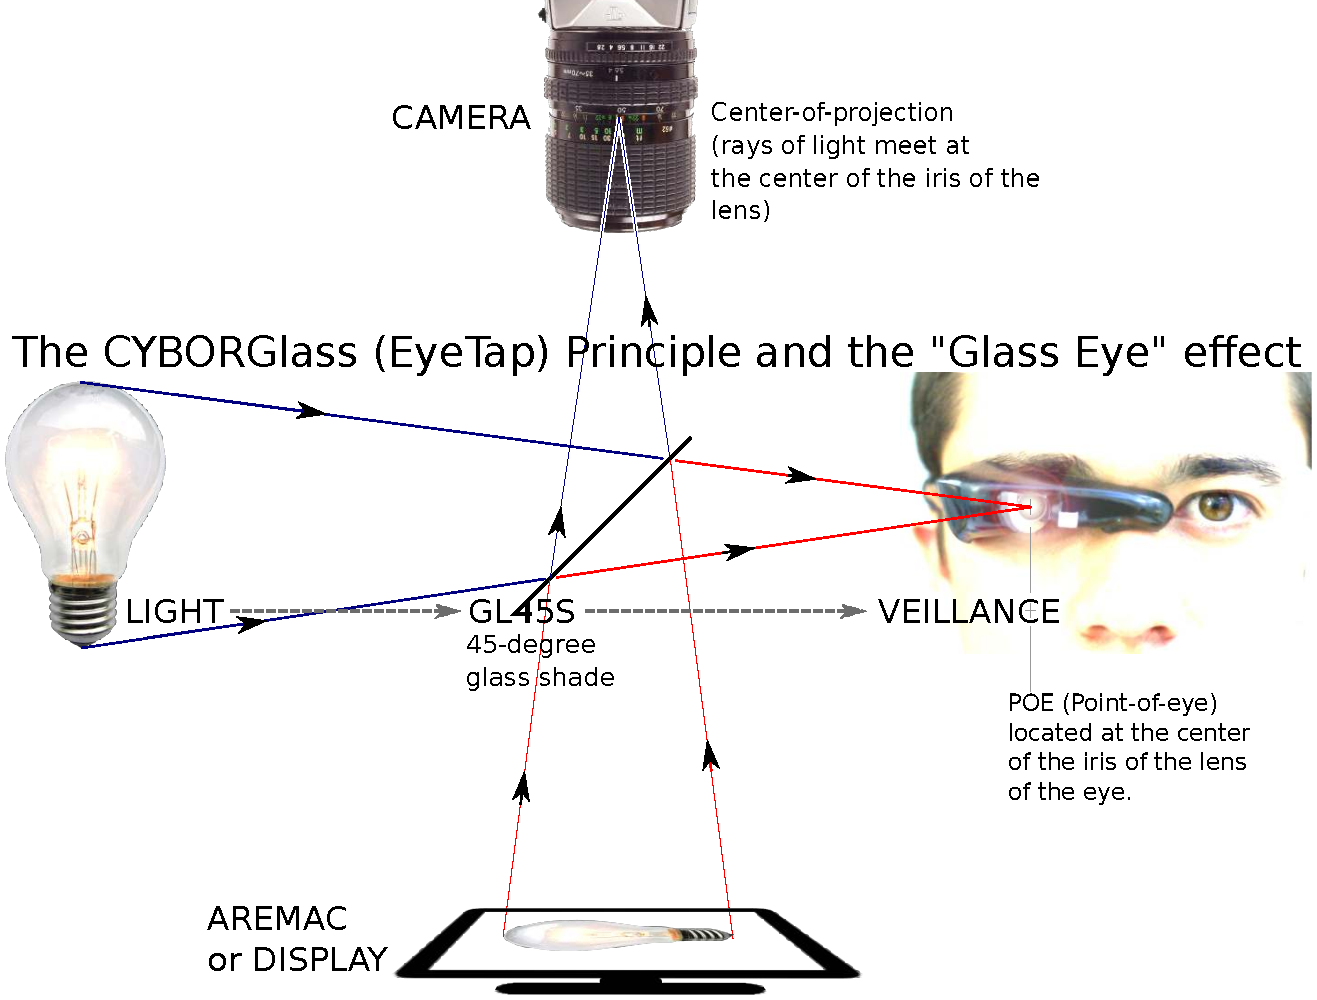
\includegraphics[width=5.0in]{ch4/diagrams/eyetap_g4_ebook.pdf}
\caption{
         Sousveillance denotes cameras worn by people.
         The ``WearCam'' Wearable Camera system, also known as
          Digital Eye Glass (DEG).
         Unlike other technologies of this era (e.g. 3M's Speedglass which
         darkens globally), the system is camera-based.
Therefore, it allows the wearer's vision to be modified
         computationally. 
         Rays of light from the subject matter (here denoted as a ``light bulb''x
         image), denoted in blue, strike a 45-degree glass shade (denoted ``GL45S''),
         arranged with a camera, such that rays of light that would otherwise
         enter the center of the iris of the eye enter the center of the iris
         of the camera.  These diverted rays are also denoted in blue.
         The camera is connected to a display system or aremac
         that re-renders the modified view of visual reality onto the backside
         of the shade (rays denoted as red lines), thus allowing the wearer
         to see in HDR Augmediated Reality.  Dark areas of the image are
         augmented, whereas bright areas are
         diminished.  Additionally computer overlays are provided.
         %The injection molded Digital Eye Glass pictured here was developed
         %for everyday use and was presented in 2002.
        % Notice how the wearer has the appearance of having a ``glass eye'',
        % hence the ``glass eye effect''\cite{presenceconnect}, hence the
        % Eye Glass is sometimes called the ``Glass Eye'' or just ``Glass''.
        }
\label{fig:deg}
\end{figure}

Sousveillance arises from Digital Eye Glass (see Fig.~\ref{fig:deg})
which itself arises from the CYBORGlass (``MannGlass'') Digital Welding
Glass (a welding shade mounted at a 45-degree angle to divert eyeward
bound rays of light into a camera system, through a wearable computer,
and then into a display system).

\section{Surveillance in the information society}
Information society is growing at a tremendous pace through
the business economy of cloud computing.
The proper working of this i-Society requires intelligent strategies in response to complex attacks~\cite{hooper2007intelligent}, as well as an effective e-Government strategy~\cite{edwards2011government}.
In addition to the need for security, there is also the need
for forensic extraction of data to meet the legitimate needs of law enforcement~\cite{olajide2011forensic}.
With mobile, portable, and personal wearable computing \cite{mann2001wearable},
there are even further security needs~\cite{fischer2012survey}.

Surveillance, together with necessary oversight mechanisms, has a
legitimate and important place in a lawful and just i-Society.
Surveillance is a well-known and, for the most-part, accepted practice.
The word ``surveillance'' is a French word that means
{\em watching} (``veillance'') {\em from above} (``sur'').
See Fig~\ref{fig:surveillance}.

The i-Society has become a ``Surveillance Society'' so
``Sureillance Studies'' is an area of increasing
importance~\cite{lyon2001surveillance}.
Surveillance is defined, formally, and precisely, as:\\
\noindent
{\tt sur-veil-lance [noun]\\
1) a watch kept over a person, group, etc., especially over a suspect,
   prisoner, or the like:
   ``The suspects were under police surveillance.''}\cite{dictionary.com}\\
Merriam Webster provides four words as synonyms for surveillance:
{\em supervision}; {\em superintendence}; {\em oversight};
{\em control}, and two
examples:
\begin{itemize}
\vspace{-.05in}
 \item ``government surveillance of suspected terrorists'';
 \item ``The bank robbery was recorded by surveillance video cameras.''.
\end{itemize}

\begin{figure*}[t!]
  \begin{subfigure}[t]{3.0in}
    \centering
    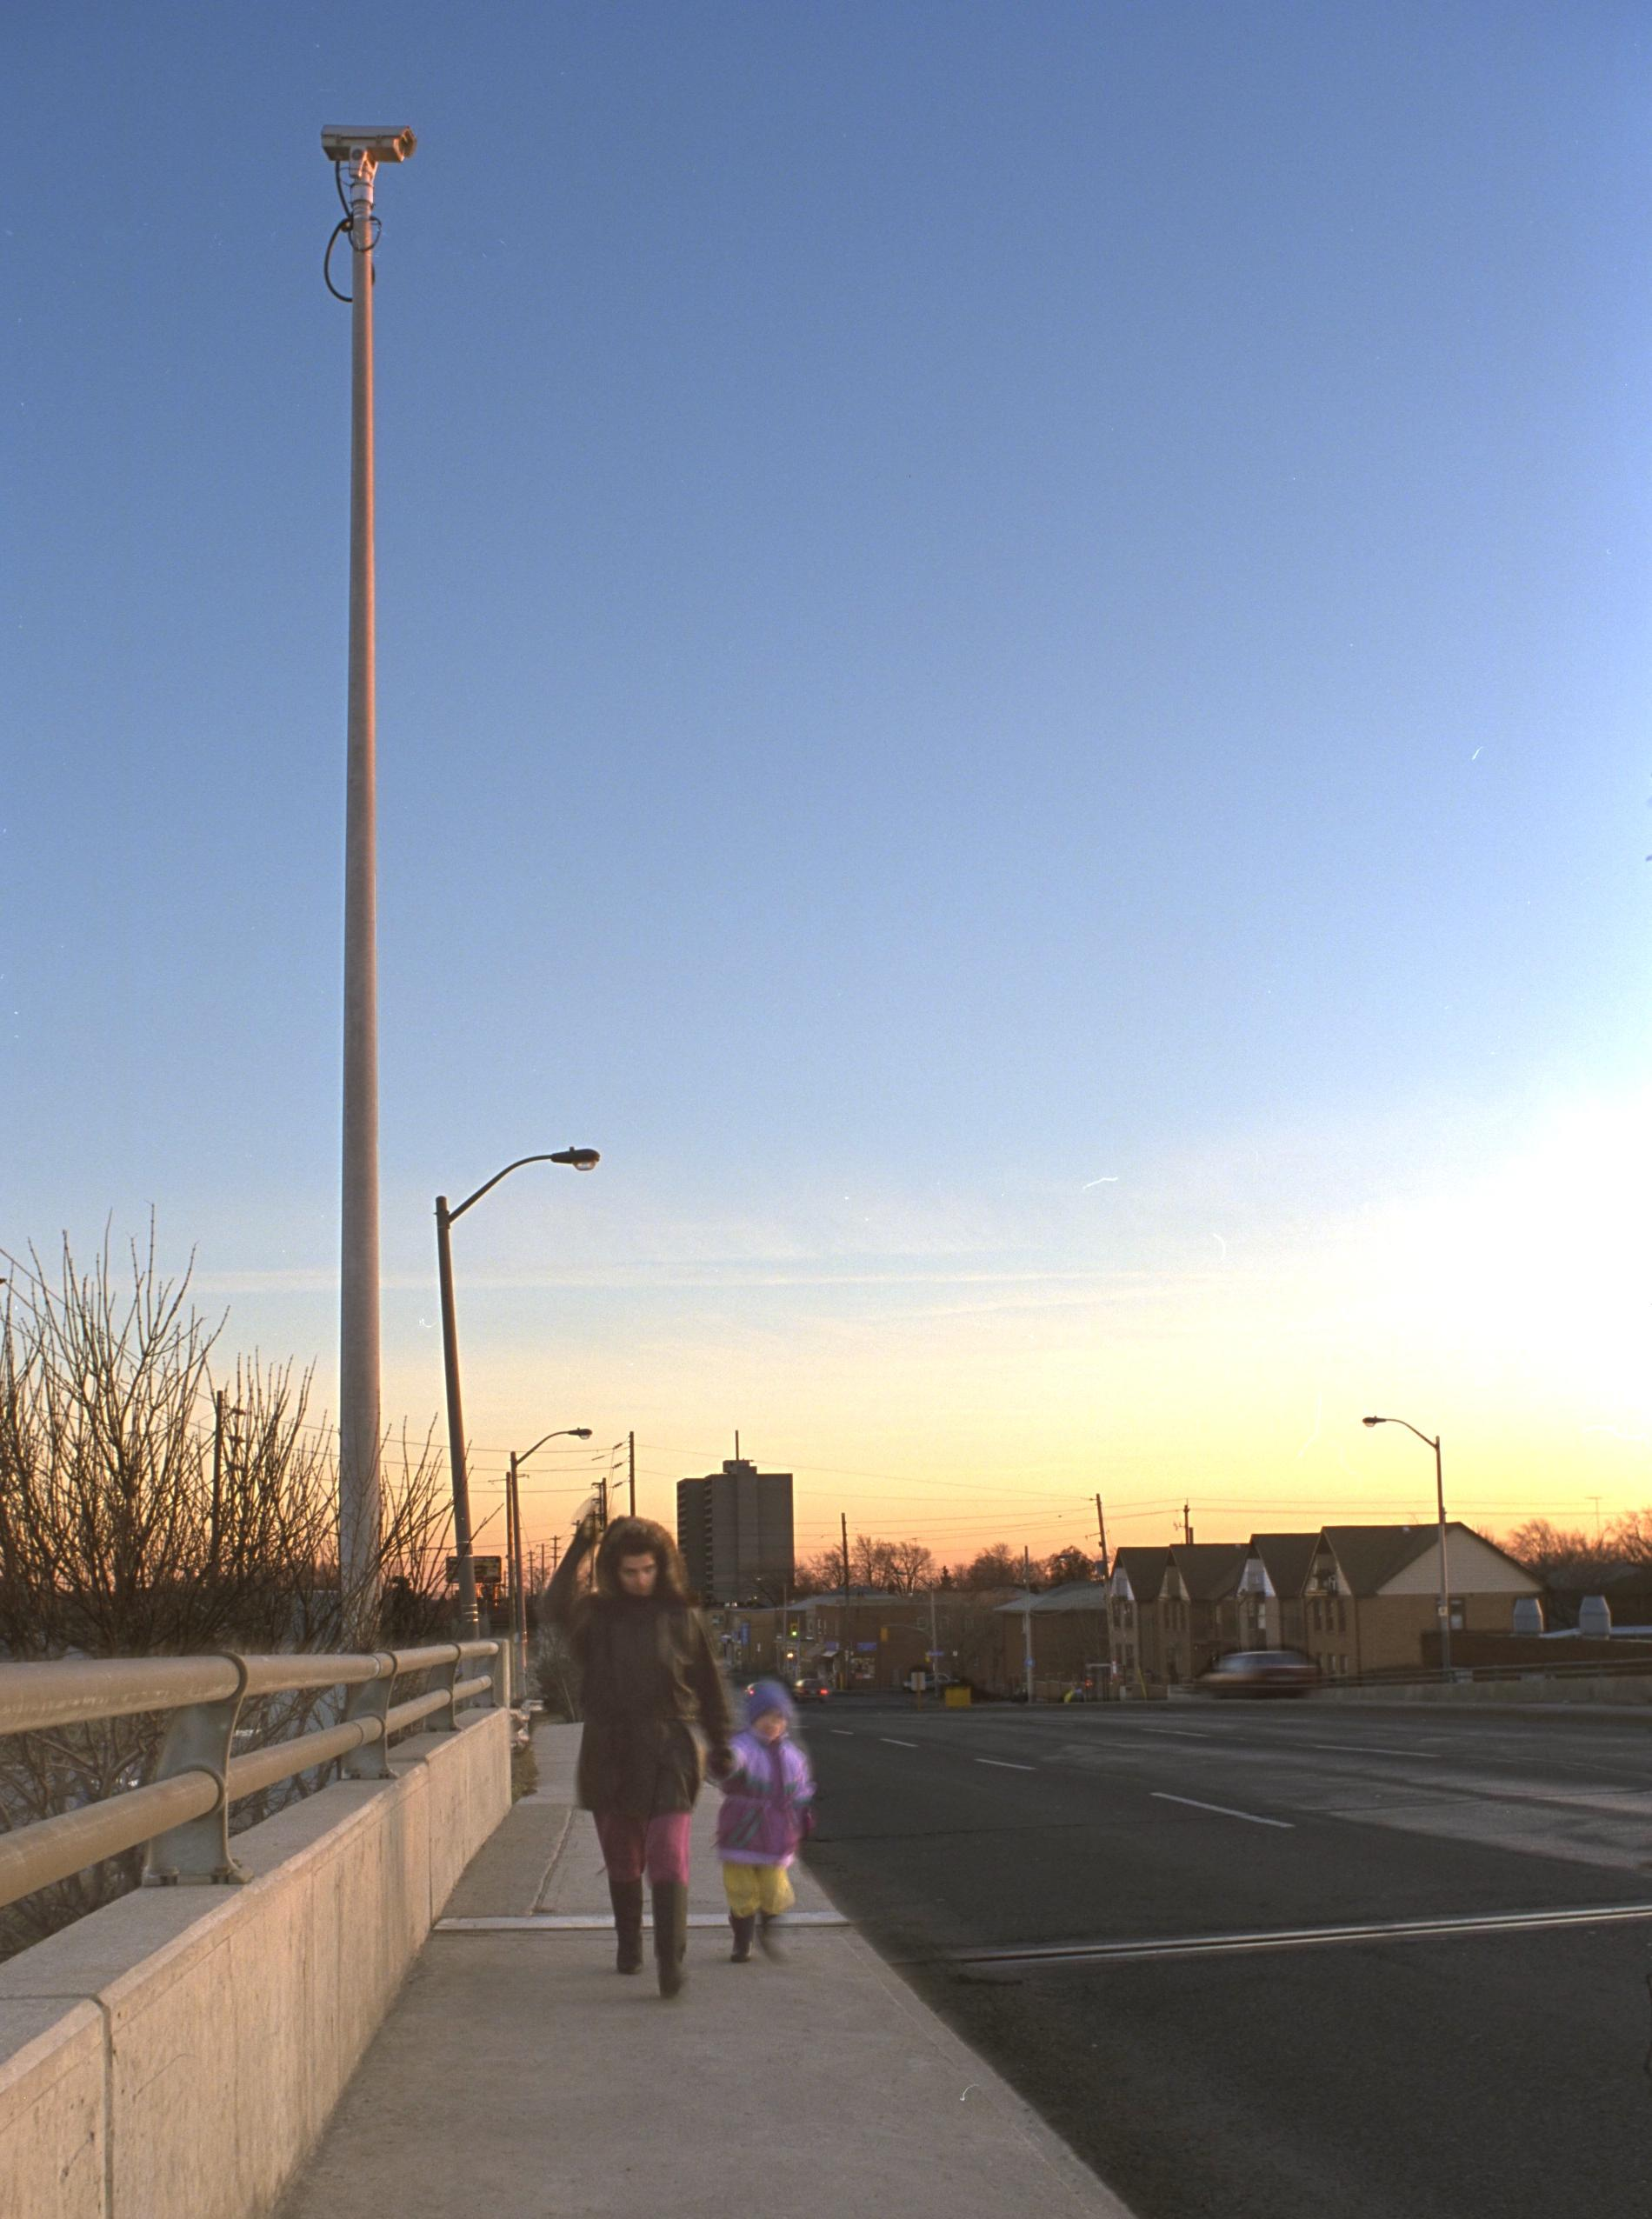
\includegraphics[height=3.0in]{ch6/figs/trafficcam.jpg}
    \label{subfig:surveillancetrafficcam}
    \caption{}
  \end{subfigure}
~
  \begin{subfigure}[t]{3.0in}
   \centering
   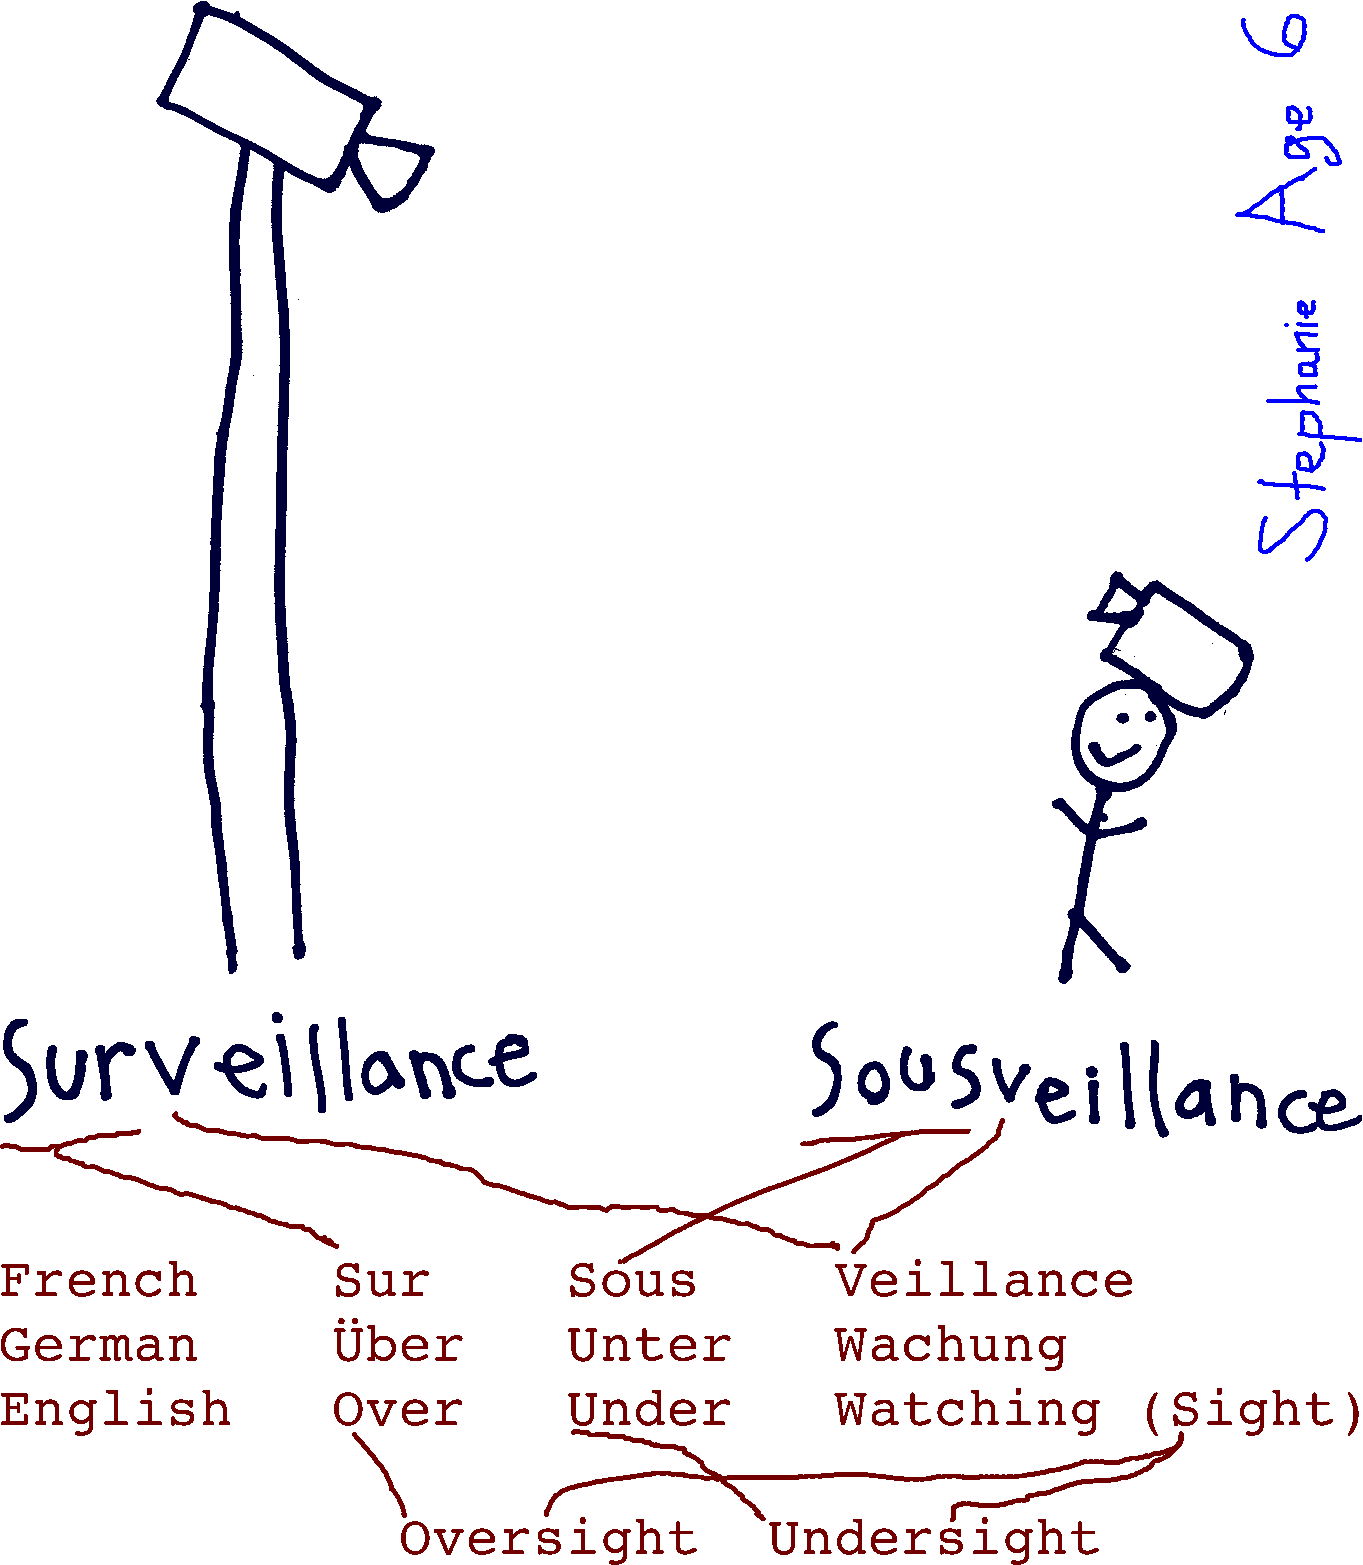
\includegraphics[height=3.0in]{ch6/figs/stephanie_sur_sousveillance_ink_drawing_words_colorized_4colors_closecrop_name.pdf}
   \label{subfig:stephanieveillance}
   \caption{}
   \end{subfigure}

%  \subfigure[]{
%   \includegraphics[height=.4in]{ch6/figs/MannGlassWBcropsmall.jpg}
%   \label{subfig:glasseye}
%  }
  %\end{subfigure}
  %~ %add desired spacing between images, e. g. ~, \quad, \qquad etc.
          %(or a blank line to force the subfigure onto a new line)
%\vspace{-0.05in}
%  A kindergarten student's drawing (Stephanie, age 6): \\
  \caption{
           (a) Surveillance camera overlooking residential area in
               Toronto, Canada.
           (b) Kindergarten student (Age 6) fluent in multiple languages draws: %\\
           %%% \\ \\\vspace{1ex}
           {\bf Surveillance}/�berwachung/Oversight =
           watching from {\bf Over} (above); and
           %\\
           {\bf Sousveillance}/Unterwachung/Undersight =
           watching from {\bf Under} (below),
           e.g. by way of a wearable camera.
  }
  \label{fig:surveillance}
\end{figure*}



%\begin{figure}
%  \includegraphics[width=3.5in]{ch6/figs/Coop1994_and_LifeGlogging_cameras_1998_2004_2013_labeled_lowres.jpg}
%  \caption{
%           A modern trend in surveillance is to conceal cameras behind
%           dark shades so that the people under surveillance cannot see
%           which way the camera is pointing, or even whether or not a
%           camera is actually present.
%           In 1998 Mann mass-produced a neckworn wearable wireless webcam
%           with fisheye lens and various sensors,
%           all concealed inside a surveillance dome adapted for being
%           neck-worn~\protect\cite{intelligentimageprocessing}.
%           The ``lifeglog'' (lifelong video record) from such cameras
%           has been used as legal evidence in physical assaults
%           and hit-and-run accidents.
%           Microsoft and Memoto later also manufactured neckworn lifeglogging
%           cameras.
%          }
%  \label{fig:domes}
%\end{figure}

%The exemplary manifestations of surveillance
%typically occur when police or guards keep watch over prisoners or suspects,
%but the prisoners or suspects often do not get to see what the police or
%guards are doing.
%Accordingly, many surveillance cameras are now concealed behind dark shades
%so that the people under surveillance cannot see which way the cameras
%are aimed, or even if one or more cameras are present (the
%dome could contain any number of cameras aimed in any number of
%directions).
%See Fig~\ref{fig:domes}.
%Thus surveillance defines a one-sided top-to-bottom gaze that gives rise to
%a one-way ``transparency''.
%
%The epitome of surveillance is a concept like Jeremy Bentham's
%Panopticon\cite{foucault}, which was the original design for prisons
%that optimized and popularized this one-sided transparency of the
%surveillance society\cite{foucault}.

Many have said that our society is rapidly becoming more like a
panoptic\cite{foucault} prison, with regards to the one-sided gaze of surveillance in which police,
governments, and private corporations are installing surveillance cameras
throughout entire cities, buildings, etc., while at the same time suspecting
anyone who takes photographs of them, or their buildings, or their
surveillance infrastructure, or the like~\cite{gandy1989surveillance}.


We live in a Surveillance Society\cite{lyon2001surveillance}
characterized by:
\begin{itemize}
 \item increased surveillance by authority figures; and
 \item the authorities' simultaneous forbidding of non-authorities from
       photography.
       See Fig~\ref{fig:signo}.
\end{itemize}


\begin{figure*} [t]
\begin{subfigure}[t]{1.5in}
   \centering
    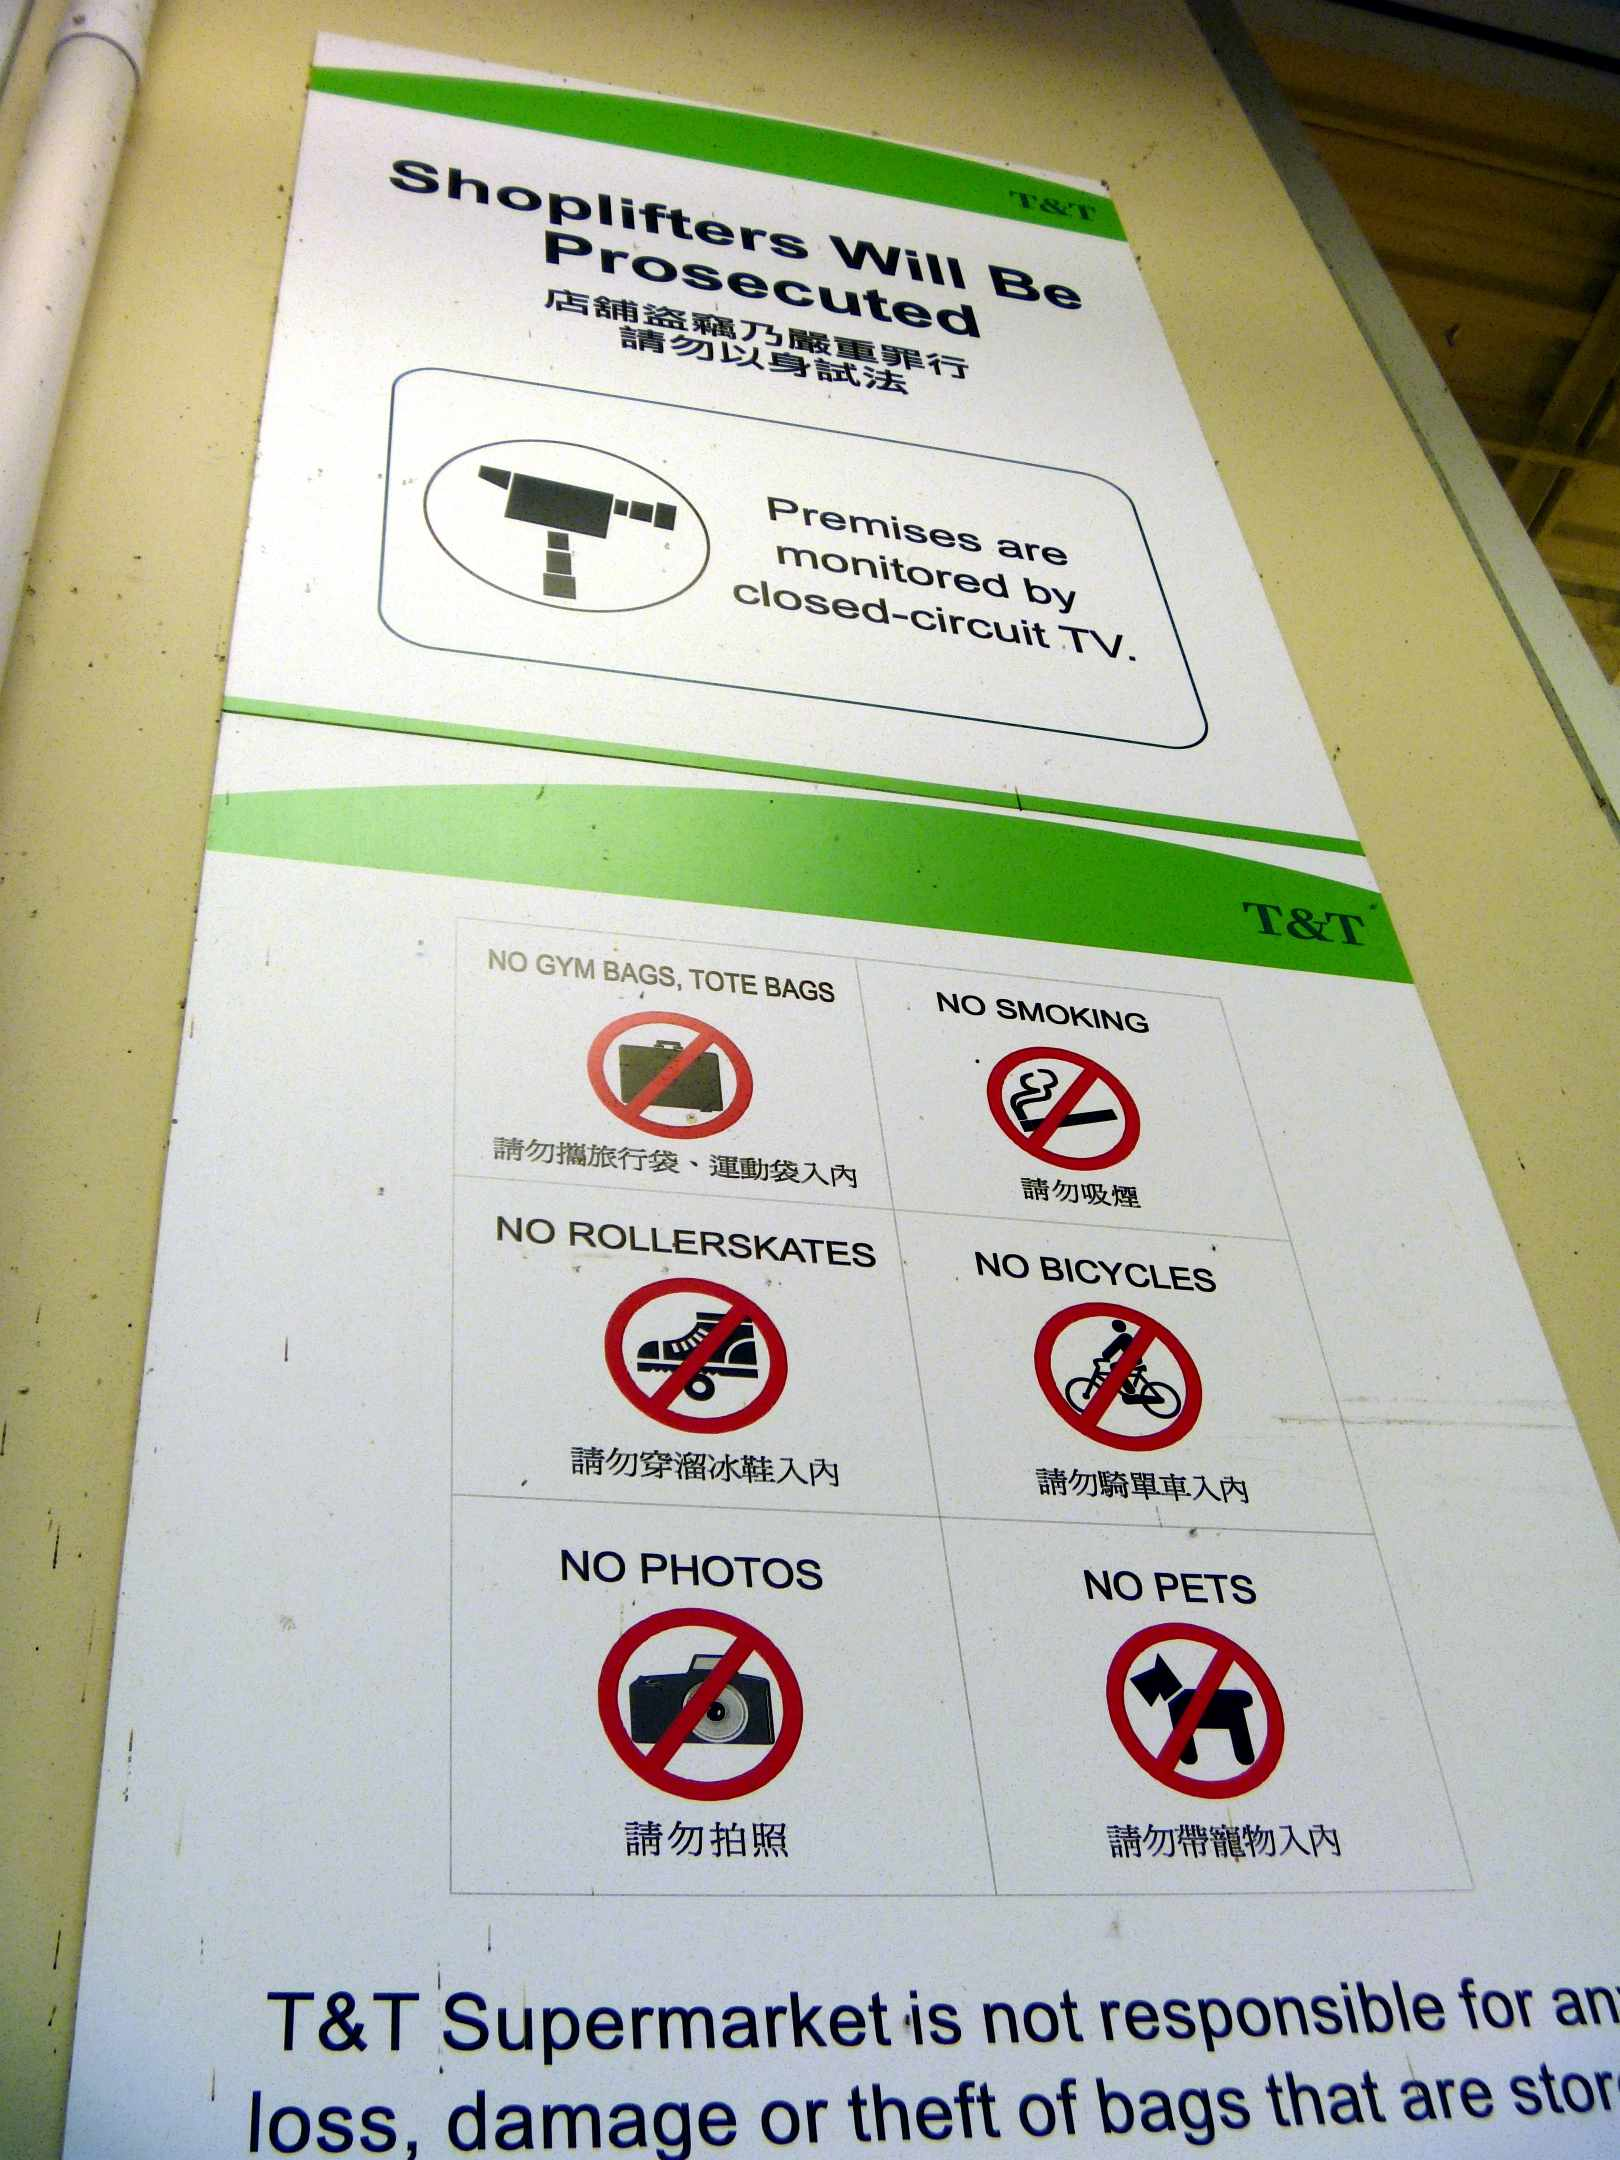
\includegraphics[height=1.3in]{ch6/figs/signo_tnt_und2.jpg}
    \caption{}
    \label{subfig:signotntwide}
\end{subfigure}
~
\begin{subfigure}[t]{3.0in}
   \centering
   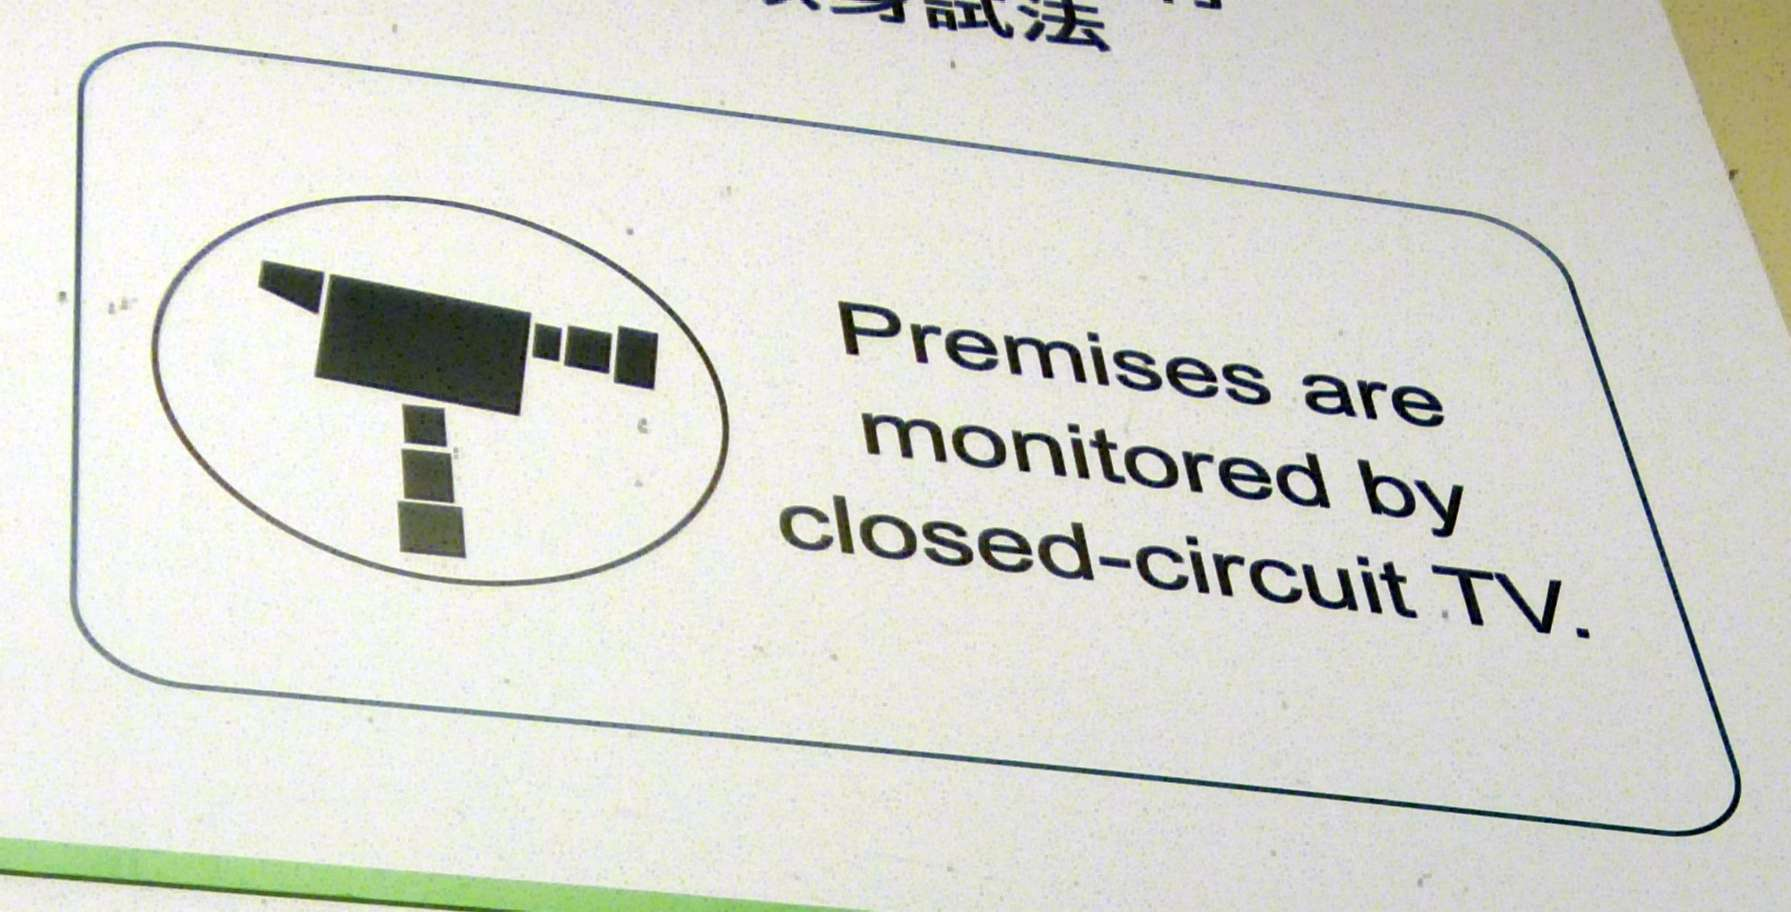
\includegraphics[height=1.3in]{ch6/figs/signo_tnt_cctv.jpg}
    \caption{}
    \label{subfig:signotntcctv}
\end{subfigure}
~
\begin{subfigure}[t]{1.5in}
   \centering
    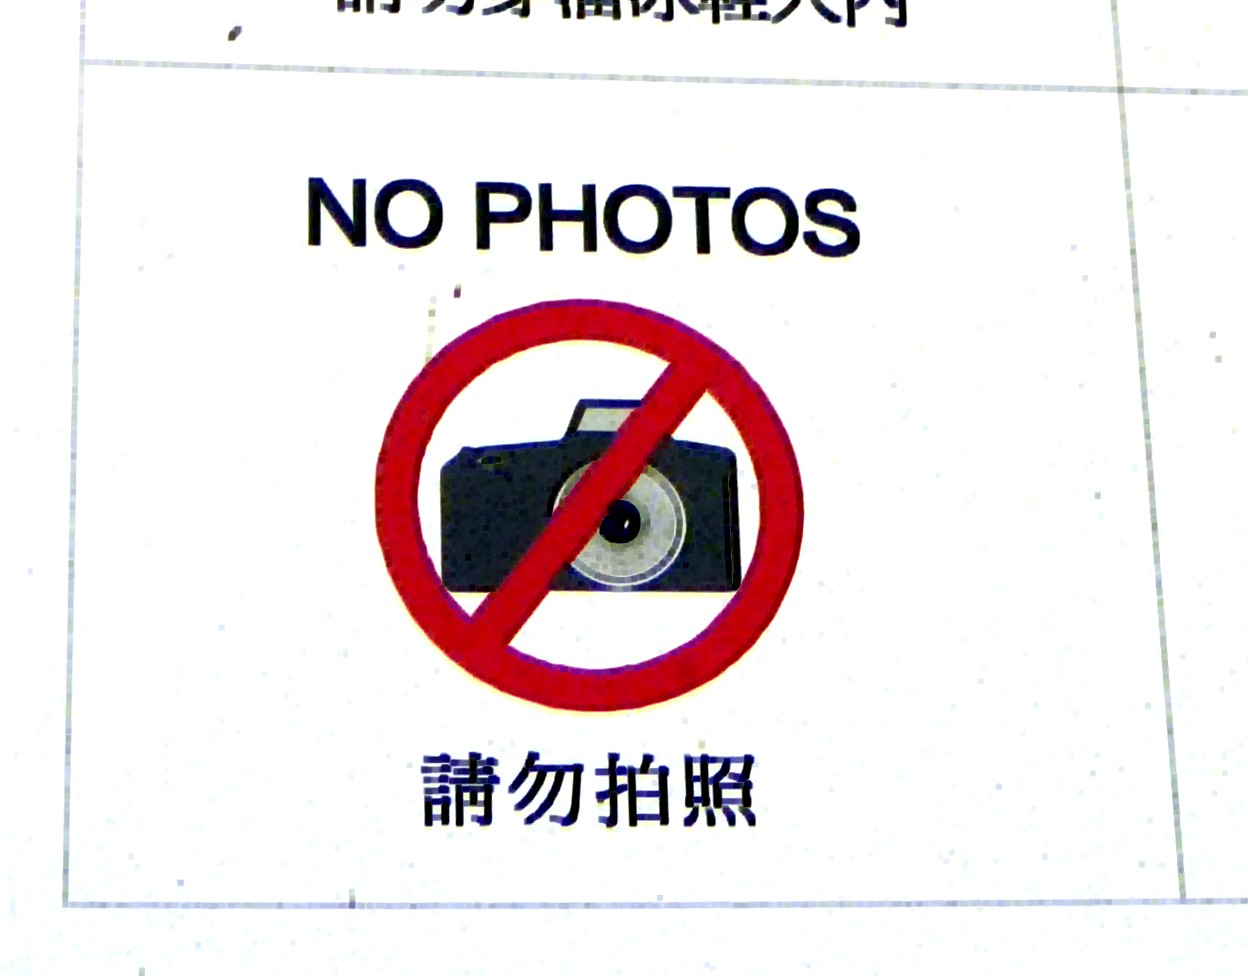
\includegraphics[height=1.3in]{ch6/figs/signo_tnt_no_photos.jpg}
    \caption{}
    \label{subfig:signotntnophotos}
\end{subfigure}

  \caption{(a) Signage at the entrance to a typical supermarket informs
               shoppers that (1) they are under surveillance (Closed Circuit
               TeleVision); and (2) that photography is prohibited.
           (b) Closeup of the sign asserting that the premises is monitored by
               CCTV.
           (c) Closeup of the sign asserting ``NO PHOTOS''.
  }
  \label{fig:signo}
\end{figure*}

Many supermarkets, while forbidding the use of smartphones,
sell products that have camera-readable barcodes (e.g. 2-D ``QR codes'') intended to give customers pre-purchase product information that will help the customers decide what to purchase.

Many buildings and other places where cameras and smartphones are forbidden
also have displays of QR codes that require cameras to read them.
See Fig~\ref{fig:qr}.

\begin{figure*}[t]
\begin{subfigure}[t]{1.5in}
   \centering
    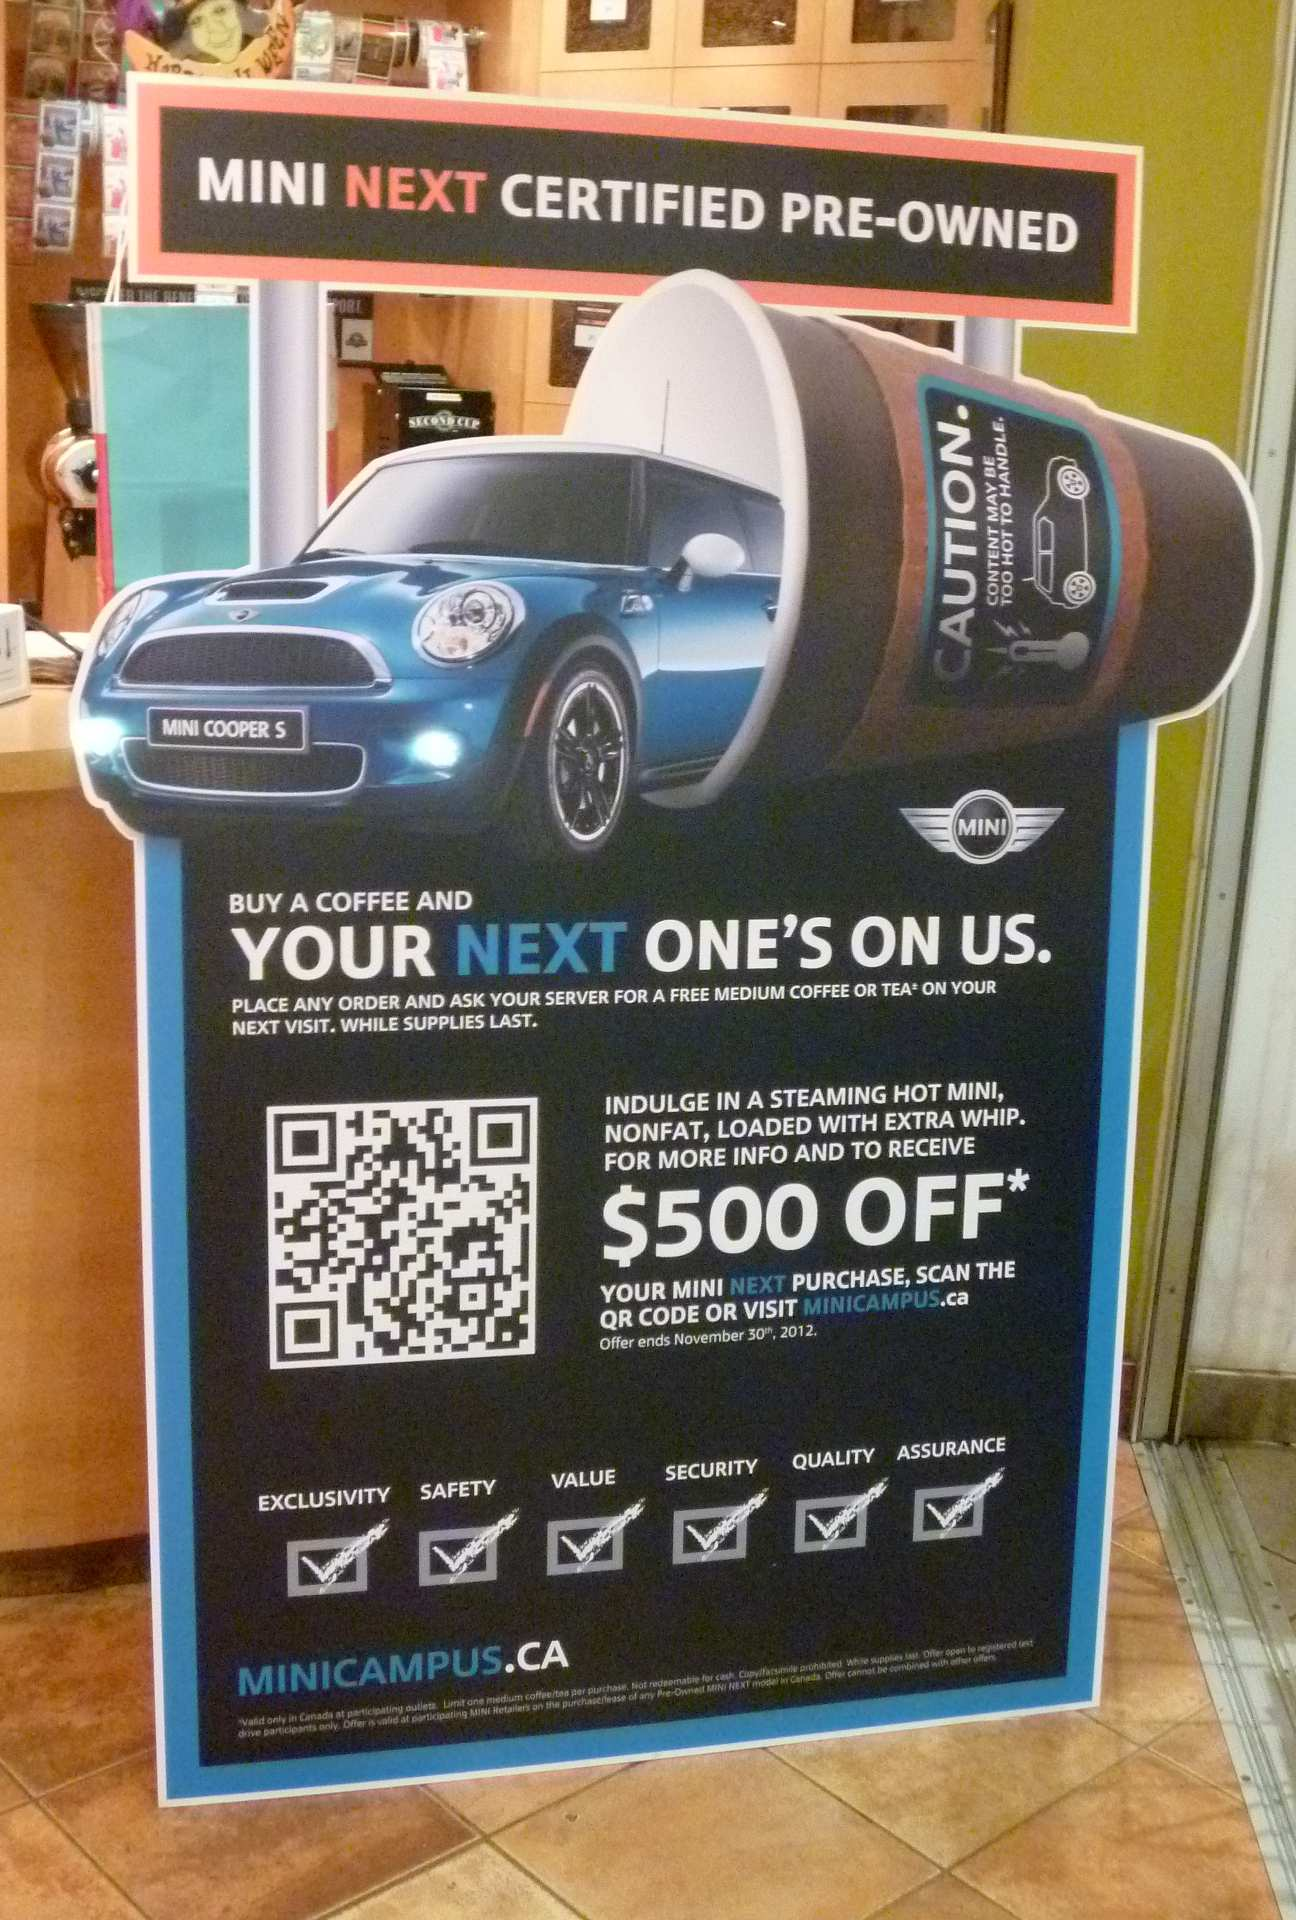
\includegraphics[height=2.0in]{ch6/figs/qr.jpg}
    \caption{}
    \label{subfig:qrwide}
\end{subfigure}
~
\begin{subfigure}[t]{4.0in}
    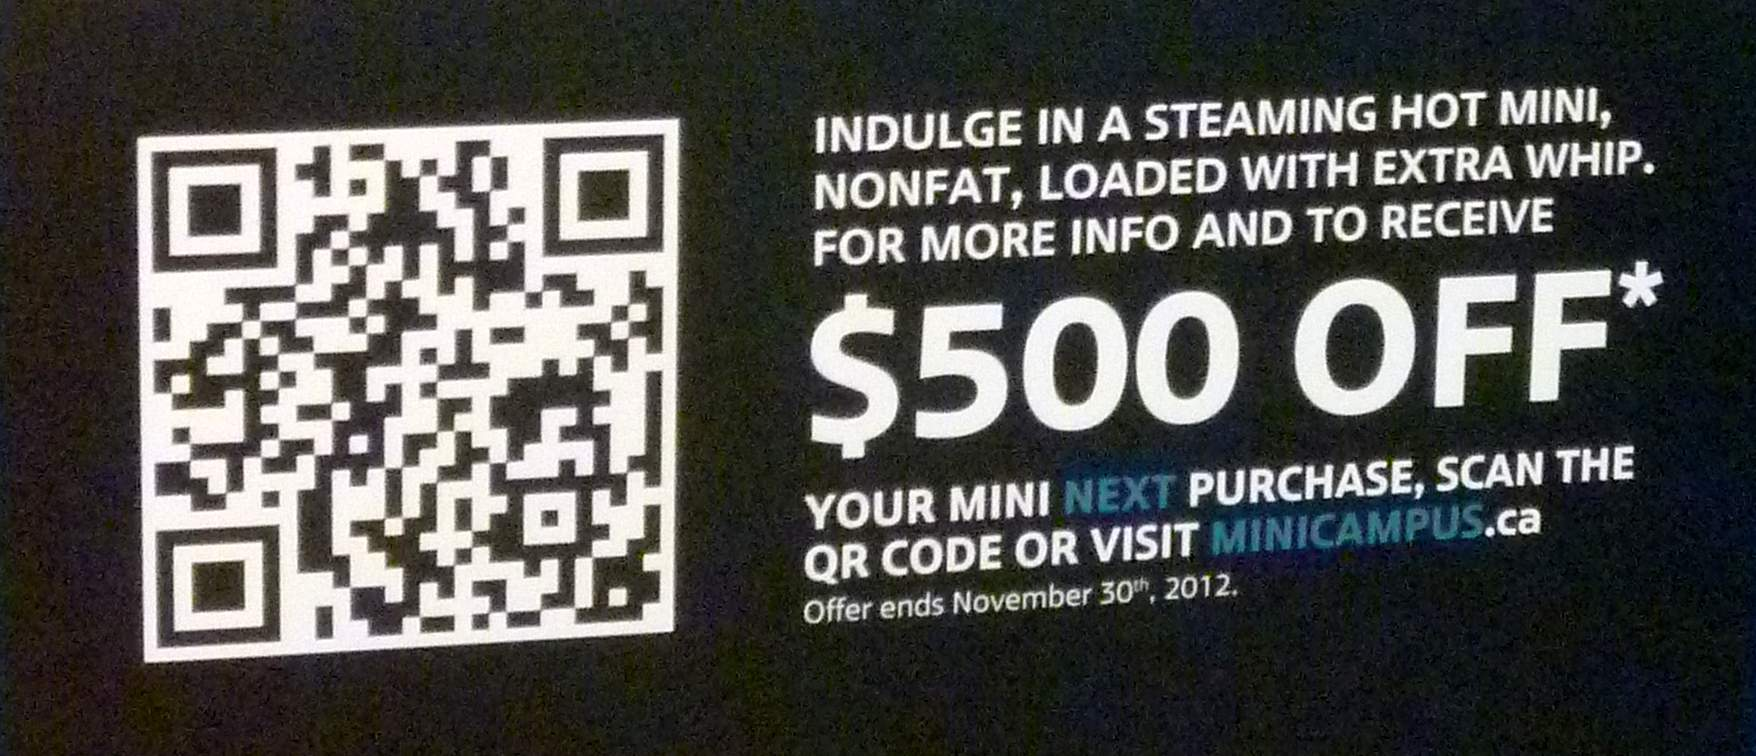
\includegraphics[height=2.0in]{ch6/figs/qr_closeup.jpg}
    \caption{}
     \label{subfig:qrcloseup}
\end{subfigure}
  \caption{(a) A massive advertisement with a QR code
               {\em in a building where cameras
               and smartphones are prohibited}.
               The act of taking this picture to document this absurdity
               was itself an act of civil disobedience.
           (b) Closeup showing the QR code, meant to be read by a camera.
  }
  \label{fig:qr}
\end{figure*}

\section{Mitigating one-sidedness of surveillance}
There are two strategies used against the one-sided nature of surveillance:
(1) activism as well as unlawful vandalism, which we do not advocate;
and (2) alternate approaches which are the subject of this chapter.
In particular, people can conduct:
\begin{enumerate}
  \item anti-surveillance (e.g. counter-surveillance, or opposing the
        surveillance).  Anti-surveillance efforts range from
        activism and legal action to illegal
        vandalism of surveillance cameras:
        \\http://camover.noblogs.org/faq/faq-in-english/
        or to simply blocking,
        covering up, or ``hacking'' sensors (``hactivism'', etc.).
        In response to these legal and illegal challenges to surveillance,
        many police departments, governments, and private companies are
        using hidden surveillance cameras, such as the cameras
        hidden inside streetlight poles throughout various cities
        [http://intellistreets.org, www.lsgc.com/pixelview/, etc.].
%        not necessarily due to privacy reasons
%, but simply the nuisance factors of sensors that malfunction when operating.
        %See Fig~\ref{fig:toilet}
  \item adding accountability to surveillance without necessarily
        opposing it.
        This may be done by:
        (2.1) wearing a display device showing current news events to help
        prevent timecode falsification by entities making surveillance
        recordings.  This approach will be discussed in Section~\ref{sec:alibi};
        or (2.2) by way of {\em sous}veillance (making one's own recording),
        also known as
        ``lifeglogging'' (lifelong cyborglogging), ``lifelogging'', or
        ``moblogging''~\cite{mann2006cyborglogging, mann2002sousveillance, fletcher2011,
                       michael2012sousveillance, bradwell2012security}.
        See Fig~\ref{subfig:stephanieveillance}.
        Sousveillance is not counter-surveillance!  In fact, methods
        (2.1) and (2.2) can be combined so that the two veillances can work
        together in a fair and balanced way, as will be described in
        Section~\ref{sec:alibi}.
\end{enumerate}

%\begin{figure}
%\noindent
%  \centering
%  \subfigure[]{
%    \includegraphics[height=2in]{ch6/figs/toiletsensorcovered.jpg}
%  }
%  \subfigure[]{
%    \includegraphics[height=2in]{ch6/figs/toiletsensorcoveredcloseup.jpg}
%  }
%  \caption{(a) Toilet sensors have evolved from a single-pixel
%               intensity-based sensor to a pixel array having
%               8 to 1024 pixels, in an active vision system, such as
%               Masco's camera-based toilet flushers (U.S. Patents 5828793
%               and 8355822).
%               These vision-based
%               sensors are often defeated by covering them with
%               toilet paper, often more due to their nuissance flushing
%               (e.g. computational errors in the computer vision algorithms)
%               than a real concern for privacy.
%           (b) Closeup picture showing placement of paper.
%  }
%  \label{fig:toilet}
%\end{figure}

%\section{Sousveillance is not counter-surveillance}
%Recently, society is experiencing a pivotal shift toward a form of
%inverse-surveillance in which widespread recording technologies are
%being used by everyday citizens to capture the actions of police and
%other authority figures.  While citizen activism has driven some of this,
%much of it is pure chance recordings by persons engaging in
%``sousveillance'', lifeglogging (lifelong cyborglogging, also known
%as ``lifelogging'', ``moblogging'' or the like)~\cite{mann2002sousveillance,
%fletcher2011, michael2012sousveillance, bradwell2012security}.
%
%Sousveillance is a more recent concept and phenomenon made possible by
%two important technological advances:
%\begin{itemize}
%  \item miniaturization of cameras and data storage technologies:
%        whereas previously cameras were large and therefore not practical
%        for being borne by small entities like individual people;
%  \item wireless communications and online connectivity: whereas previously,
%        cameras often had to be wired for both power supply and data
%        (analog or digital) communications, making it less practical to
%        be borne by a moving rather than stationary entity.
%\end{itemize}
%
%The word ``sousveillance'' comes from replacing the ``sur'' (which
%means ``above'') with ``sous'' (which means ``below''), as the prefix to
%the word ``veillance'' (which means ``watching'')~\cite{mann2002sousveillance,
%fletcher2011, michael2012sousveillance, bradwell2012security}.
%See Fig~\ref{subfig:stephanieveillance}.

%Table~\ref{tab:veillances} outlines these etymological differences between
%surveillance and sousveillance.
%\begin{center}
%\begin{table}[b]
%\vspace{-0.075in}
%\centering
%\normalsize
%\begin{tabular}{ll} \toprule
%English                                     &  French       \\
%\midrule
%{\bf to watch}                              &  {\bf veiller}      \\ 
%\cmidrule(lr){1-2}
%{\bf watching} (monitoring)                 &  {\bf veillance}    \\
%\cmidrule[\lightrulewidth](lr){1-2}
%{\bf oversight (watching over)}             &  {\bf surveillance} \\ 
%\cmidrule(lr){1-2}
%{\bf to oversee} (to watch from above)      &  {\bf surveiller}   \\ 
%\cmidrule(lr){1-2}
%{\bf over} (from above)                     &  {\bf sur}   \\ 
%\cmidrule[\lightrulewidth](lr){1-2}
%{\bf under} (from below)                    &  {\bf sous}   \\ 
%\cmidrule(lr){1-2}
%{\bf ``undersight''} (to watch from below)  &  {\bf sousveillance} \\ 
%\bottomrule
%\end{tabular}\\
%\hspace{.1in}
%  \caption{The Veillances: SurVeillance and SousVeillance
%           \label{tab:veillances}
%          }
%\end{table}
%\end{center}

\begin{figure*}
\center
\begin{subfigure}[b]{5.0in}
%  \includegraphics[height=1.6in]{ch6/figs/GL455proccrop_lowres.jpg}
  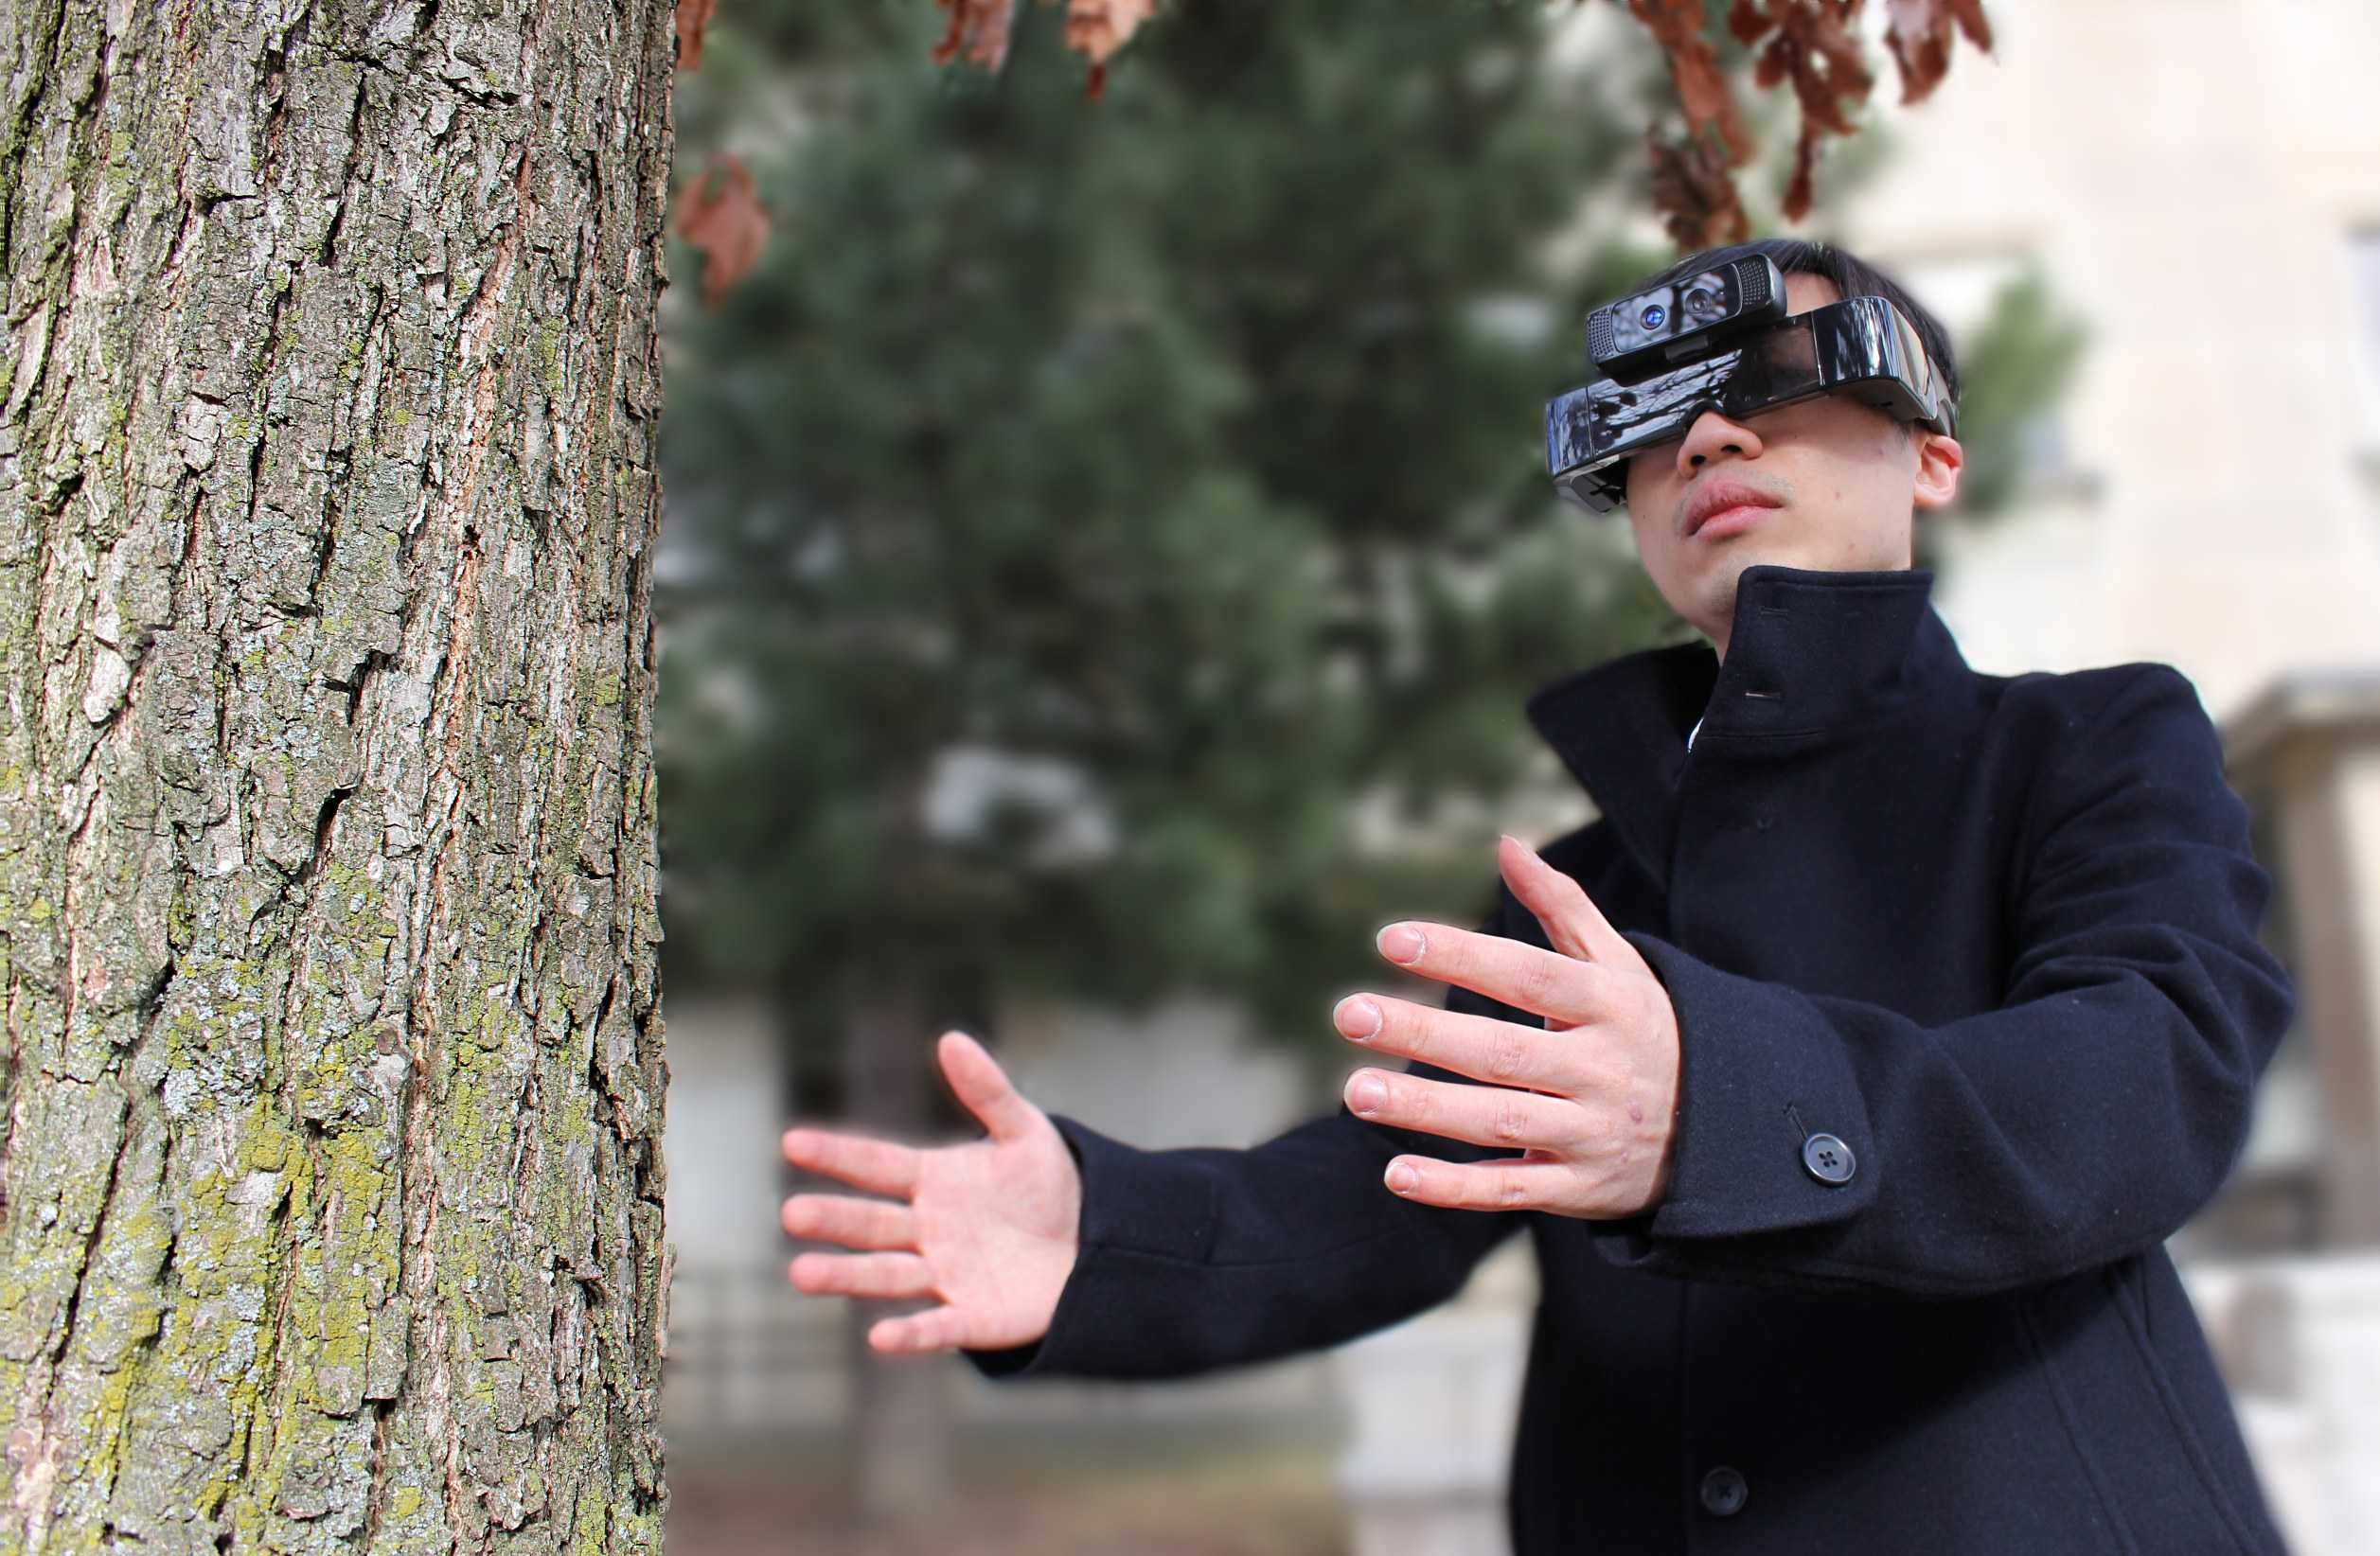
\includegraphics[width=5.0in]{ch6/figs/GL4S5_whiteoak_treehug_gesture_cropped.jpg}
  \caption{}
\end{subfigure}

\begin{subfigure}[b]{2.5in}
  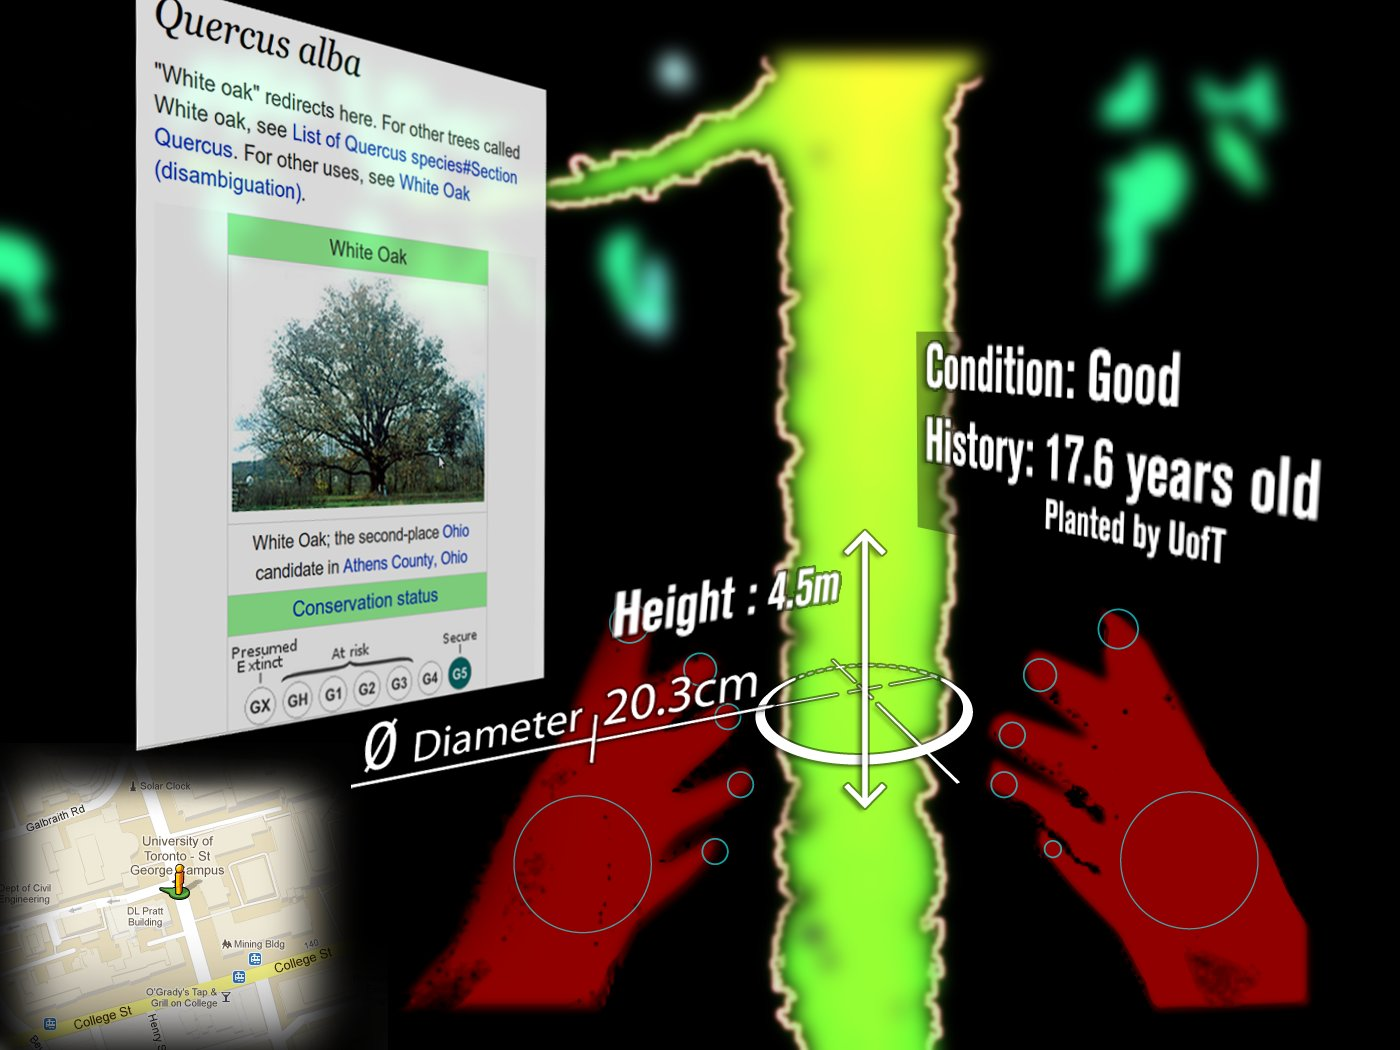
\includegraphics[width=2.5in]{ch6/figs/treePrompt2OverlayOnly.jpg}
  \caption{}
\end{subfigure}
~
\begin{subfigure}[b]{2.5in}
  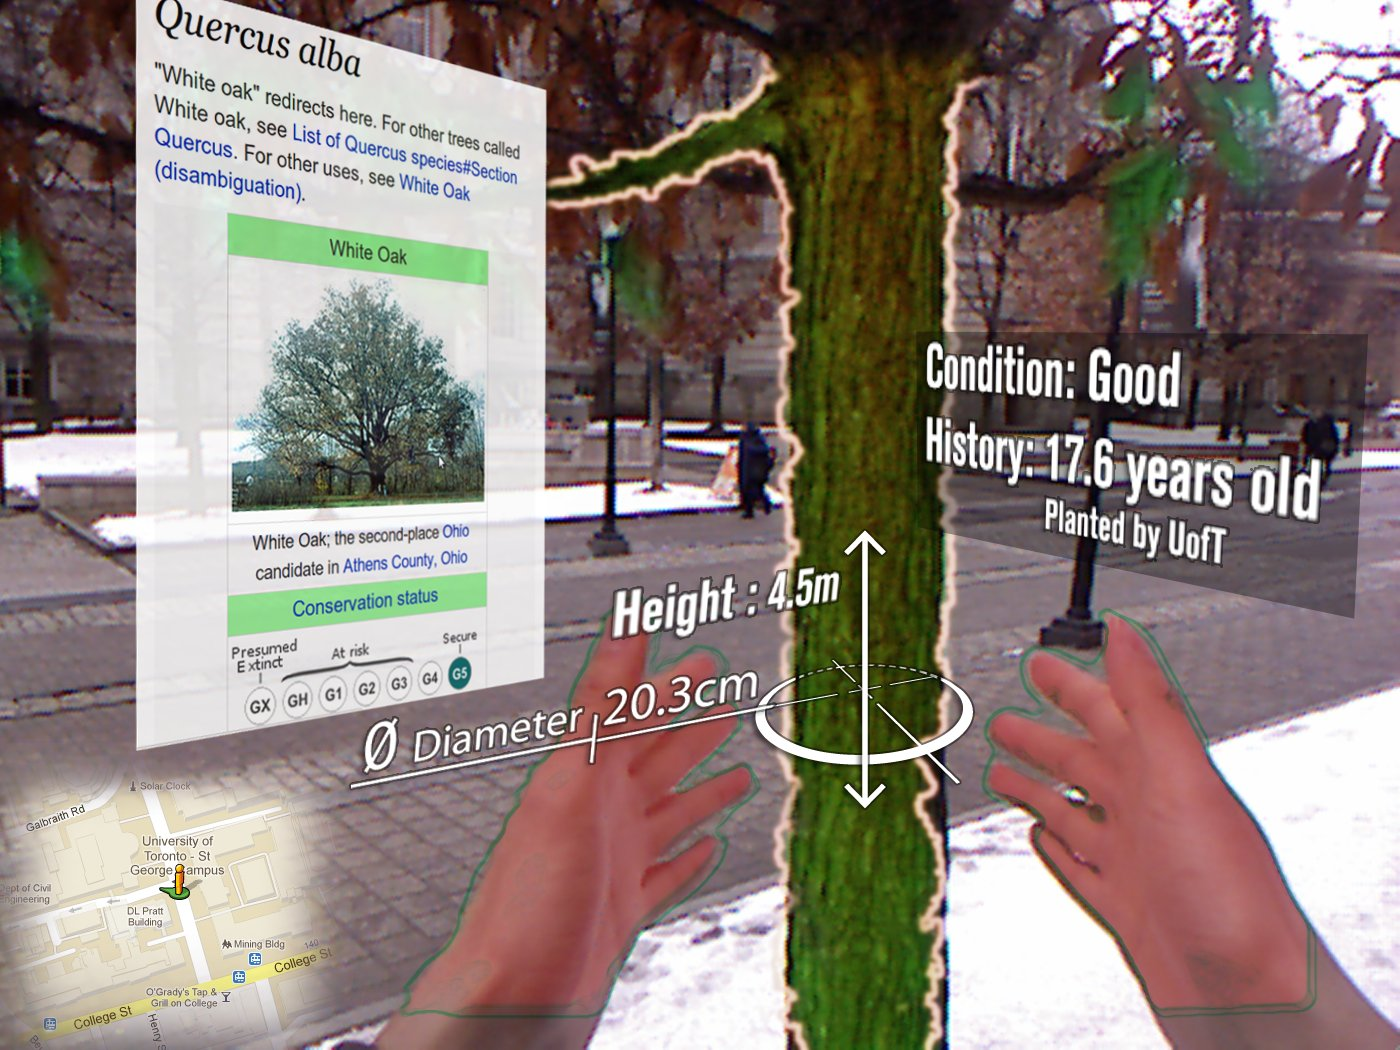
\includegraphics[width=2.5in]{ch6/figs/treePrompt2.jpg}
  \caption{}
\end{subfigure}

  \caption{(a) A practical implementation of the Generation-5 Glass: A stereo
           vision display with a true time-of-flight 3D camera system.
           (b) Hand gesture automatically recognized along with automatic detection of the subject matter (tree).
           The hands and subject matter (tree) were segmented from the scene using depth
           information captured by the 3D sensor.
           (c) Information retrieved and overlaid onto the
           stereo display in real-time. Overlays are rendered next to the
           subject matter for ease of reading/viewing. 
           }
  \label{fig:treehugger}
\end{figure*}


\subsection{Sousveillance versus surveillance with 3D cameras}
Surveillance is an application where cameras are affixed to the environment,
so there is no relative movement between the camera and the static
objects in the background.
But with sousveillance, the camera is affixed to a person, thus causing
relative movement between the camera and static background objects.
For this reason, computer vision for
sousveillance is a much harder problem than for surveillance, where all we
need to do is subtract the background.

However, 3D sensing cameras, originally designed for surveillance
(being fixed to architectural elements like a shelf in a living room for
example), can be applied to sousveillance.

In particular, an important observation to make is the 3D camera's ability
to ignore subject matter beyond a certain distance from the camera.
In this way, the 3D camera can distinguish between gestures and near-field
subject matter and background clutter.
For this reason, 3D cameras are more well suited to sousveillance than
the surveillance they were designed for~\cite{mann2011blind}.

Wearing the 3D camera gives a setup optimized for near-field time-of-flight sensing
of hand gestures at close range, while ignoring the background --- a task
that has previously been very difficult with 2D wearable camera systems.
Background clutter is eliminated from the scene by simply determining
which areas of the image that are beyond the depth range of the sensor.

%\begin{figure}
%  \includegraphics[height=1in]{ch6/figs/6ense_und2.jpg}
%  \caption{6ense: Synthetic Synesthesia of the Sixth Sense}
%  \label{fig:6ense}
%\end{figure}
\section{Applications}
We present two applications of the Gen-5 Glass:
\begin{itemize}
  \item Reality User Interface;
  \item ``ALIBEye: Eye Was Here''.
\end{itemize}

\section{Reality User Interface}
Unlike the typical GUI (graphical user interface) found in desktop computing,
or mobile devices, our system requires only simple gestures, such as the
``Outstretched-Hands'' gesture in front of any subject matter,
as shown in Fig.~\ref{fig:treehugger}.
This enables the seamless interaction between the physical world and
Digital Eye Glass.
For example, reaching out to a tree, the tree ``answers back'' with
information about itself.  Although the Landscaping Department has a
database of all trees planted, and thus the knowledge could be obtained
``top-down'' (i.e. from the authorities), our application allows individuals
to acquire, disseminate, and share knowledge in a ``bottom-up'' way,
 through shared sousveillance.  The 3D camera in the eyeglass collects
information about the environment, enabling individuals to be producers of
--- and not merely consumers of --- information.
Thus, the proposed Gen-5 Glass answers the call of ``hacccessibility'',
i.e. the DIY (Do-It-Yourself) spirit of community-based knowledge
acquisition during and about everyday life activities, such as enjoying nature.


\section{Alibi sousveillance}
\label{sec:alibi}
Our second application is called ``ALIBEye: Eye Was Here''.
It provides a lifeglogging experience that can be used as an alibi,
in a court-of-law, for example, to prove one's time and place.
%identifeye, etc..

One way of mitigating the one-sided nature of
surveillance is to hold those doing the surveillance accountable.
This can be done by sousveillance (keeping one's own recording of what
happens).  In this case, it is useful to timestamp one's own sousveillance
recordings so that they can be used as an alibi in any accusation of wrongdoing.
Another way of mitigating the one-sided nature of surveillance is to
timestamp the surveillance data.  This can be done without the consent of ---
and even against the will of --- the authorities conducting the surveillance.
An example of this is the display of content into the surveillance data.
For example, if you simply walk around with a copy of the front page of
a newspaper, and display it to every surveillance camera you see, you've
greatly reduced the ability of the authorities to backdate the
surveillance video (See Fig~\ref{fig:proj_ray}).  Wearing a small 2D bar-code
that updates with a hash of the day's news headlines, for example, can serve
a similar effect.

Ideally a combination of these two methods can be used, in which one
records one's own sousveillance video, while also displaying to one's self
AND to other cameras (other sousveillers and the surveiller), a hash of
today's latest news, and then time stamping that sousveillance recording.

%A community of users who operate in this way can moreover create a
%``web of veillance'' that is far more trustworthy than a single
%surveillance authority with its own (easily falsifiable) timestamping.

The use of a visual recording to provide an alibi requires that the time of
recording is bounded both before AND after the recording takes place.
Standard cryptographic time-stamping of a hash of a digital recording
provides evidence that the recording took place \emph{before} the
timestamp; i.e. the signed hash depends on the recording.
We now describe approaches to bound the time of recording in
the other direction, providing evidence that the recording took place
\emph{after} a certain time, preventing replay attacks, and preventing
temporal falsification in BOTH temporal directions.

Alibi veillance can be used for both surveillance and sousveillance and
in various combinations of these veillances.

%\subsection{Alibi veillance example: The Myers murder}
%Question: Suppose you're going about your daily life wearing a
%sousveillance device
%(e.g. uploading + timestamping pictures or video),
%and a murder is committed, in which you
%are the prime suspect.  You say, ``I have timestamped images of where
%I was that day!''.  Will you be exonerated?  No, not necessarily...
%
%Something similar to this actually happened, in 1997 on October 20th.
%In York, PA, USA, a woman names Jennifer Myers was murdered.  The
%prime suspect, Kevin Brian Dowling, had videotaped himself fishing
%that same day, and in this way the recording was explored as an electronic
%alibi: the video camera put a visible time-date stamp on each
%video frame.  He also appeared a bit earlier in the security videos of
%local bait and tackle shops.  However, a forensics expert determined a
%time-shift in the video of several hours, due to the position of the
%sun in the sky.
%In fact, Dowling had merely adjusted the clock on the camera by
%around three hours (perhaps in an attempt to provide himself with an alibi,
%or perhaps it was an accidental error).
%
%This discrepancy was only caught by the position of
%the sun.  So if the timestamp had been off by exactly 24 hours, or
%exactly one year (same day and time-of-day),
%when the sun was in almost perfect alignment with the
%target time, this discrepancy might never have been noticed.
%
%The problem with local timestamps is that they are easily falsified,
%or a non-deliberate error can also occur and not be detected.
%
%A remote timestamp can only attest to the time of upload, not capture.
%That is, a server timestamp prevents backdating, but not postdating.
%Something obvious, like looking at a newspaper headline, can prove
%that a video is not  postdated. This his is a well-known trope of kidnappers
%and terrorists~\cite{onion2009}, or anyone else with hostages that
%they wish to prove are still alive on a certain day.  But the newspaper
%method is inconvenient for automation of the process.
%
%Looking at a television broadcast with a stock-ticker would narrow down
%the time-windowgreatly since the video capture must have been between
%the time a stock symbol hit a certain value (or better yet, a sequence
%of symbols, to ensure uniqueness) and the time the timestamp server
%accepted the image hash upload.  Looking at a clock does not help at
%all, since they are easily falsified or accidentally erroneous
%by being set to a different
%time, as with Dowling's video.  A sophisticated video-editing program could
%even be employed, to make such changes automatically.
%
%The qualities that make newspaper headlines a kidnapper's favorite are
%that they are published frequently,typically not predictable, and
%are widely observed and therefore easily and independently verifiable
%by other parties.

\subsection{Prior work: Timestamps are all one-sided}
A digital timestamp can prove to the world that a certain set of bits
existed before a certain time, namely when the timestamp was
created~\cite{schneier1995}; examples are
formalized in IETF's RFC 3161~\cite{rfc3161}, RFC 3339~\cite{rfc3339}, and
ANSI's X9.95~\cite{ansi-x9.95}.

\subsection{Alibi Veillance: Another side to time-stamping}
To create an alibi veillance system,
three elements are required: ($A$) an \emph{a priori} unknowable
fact that is widely observed, ideally in a precise digital form; and
($B$) a way to embed $A$ into a real-world scene, and record the
embedding, in a way that is very
difficult to falsify; and ($C$) a verifiable
timestamp service, to which a hash of the recording is can be immediately
submitted to.

Steps A and B bound the time in one direction, and step C bounds it in the
other temporal direction, thus resulting in a bi-directional bounding of the
alibi veillance.

\subsection{Alibi displays}
A simple embodiment of this idea is to display a hash of current events,
as a QR code.  This can be done, for example, on a GNU Linux wristwatch
that runs a ``cron job'' to automatically display the material now and 
again, so as to be visible to the wearer of a sousveillance eyeglass,
or other wearable camera that can view the wristwatch (as well as other
cameras in the environment, including surveillance cameras, being able
to view the wristwatch).
See Fig~\ref{fig:wristcomp}.
\begin{figure*}[t]
\center
\begin{subfigure}[t]{4.0in}
   \centering
    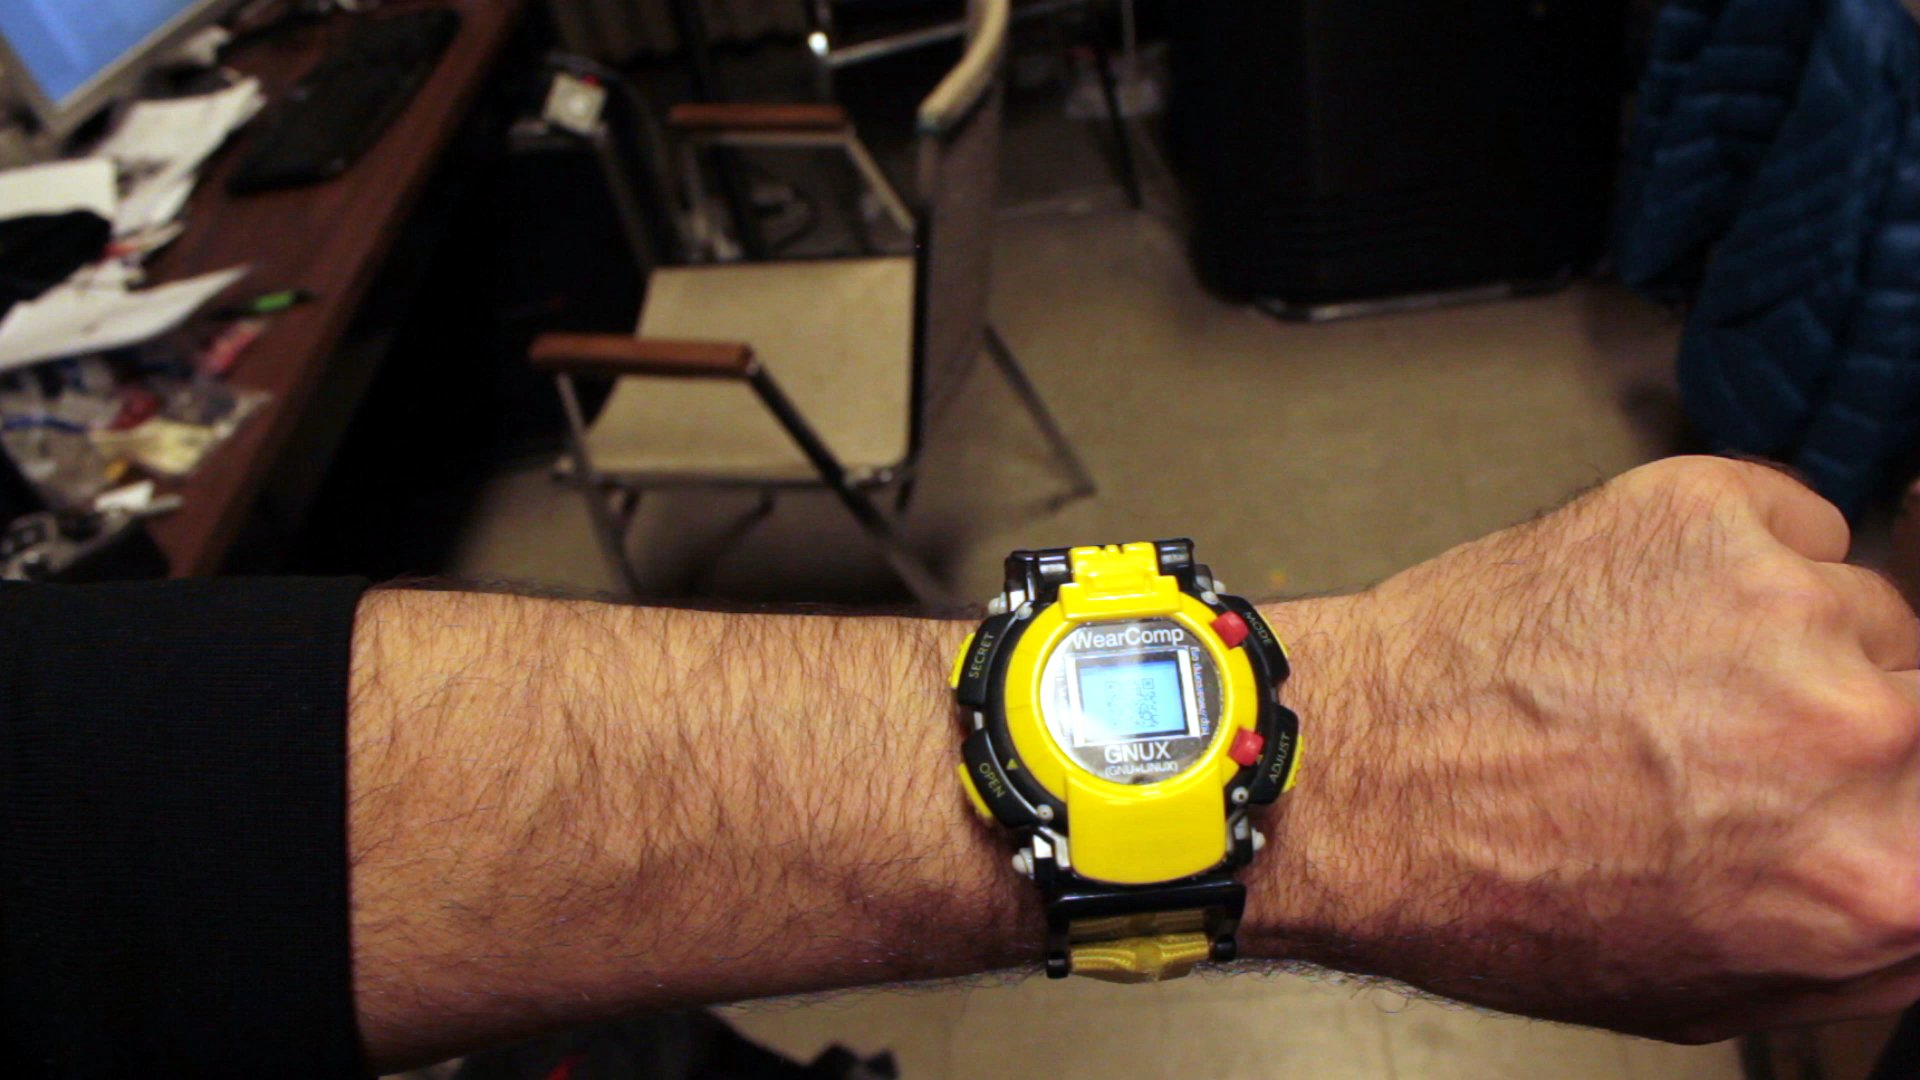
\includegraphics[height=2.0in]{ch6/figs/wristcomp1.jpg}
    \caption{}
    % \includegraphics[height=.9in]{ch6/figs/wristcomp2.jpg}
    \label{subfig:wristcomp}
\end{subfigure}
\begin{subfigure}[t]{2.0in}
   \centering
    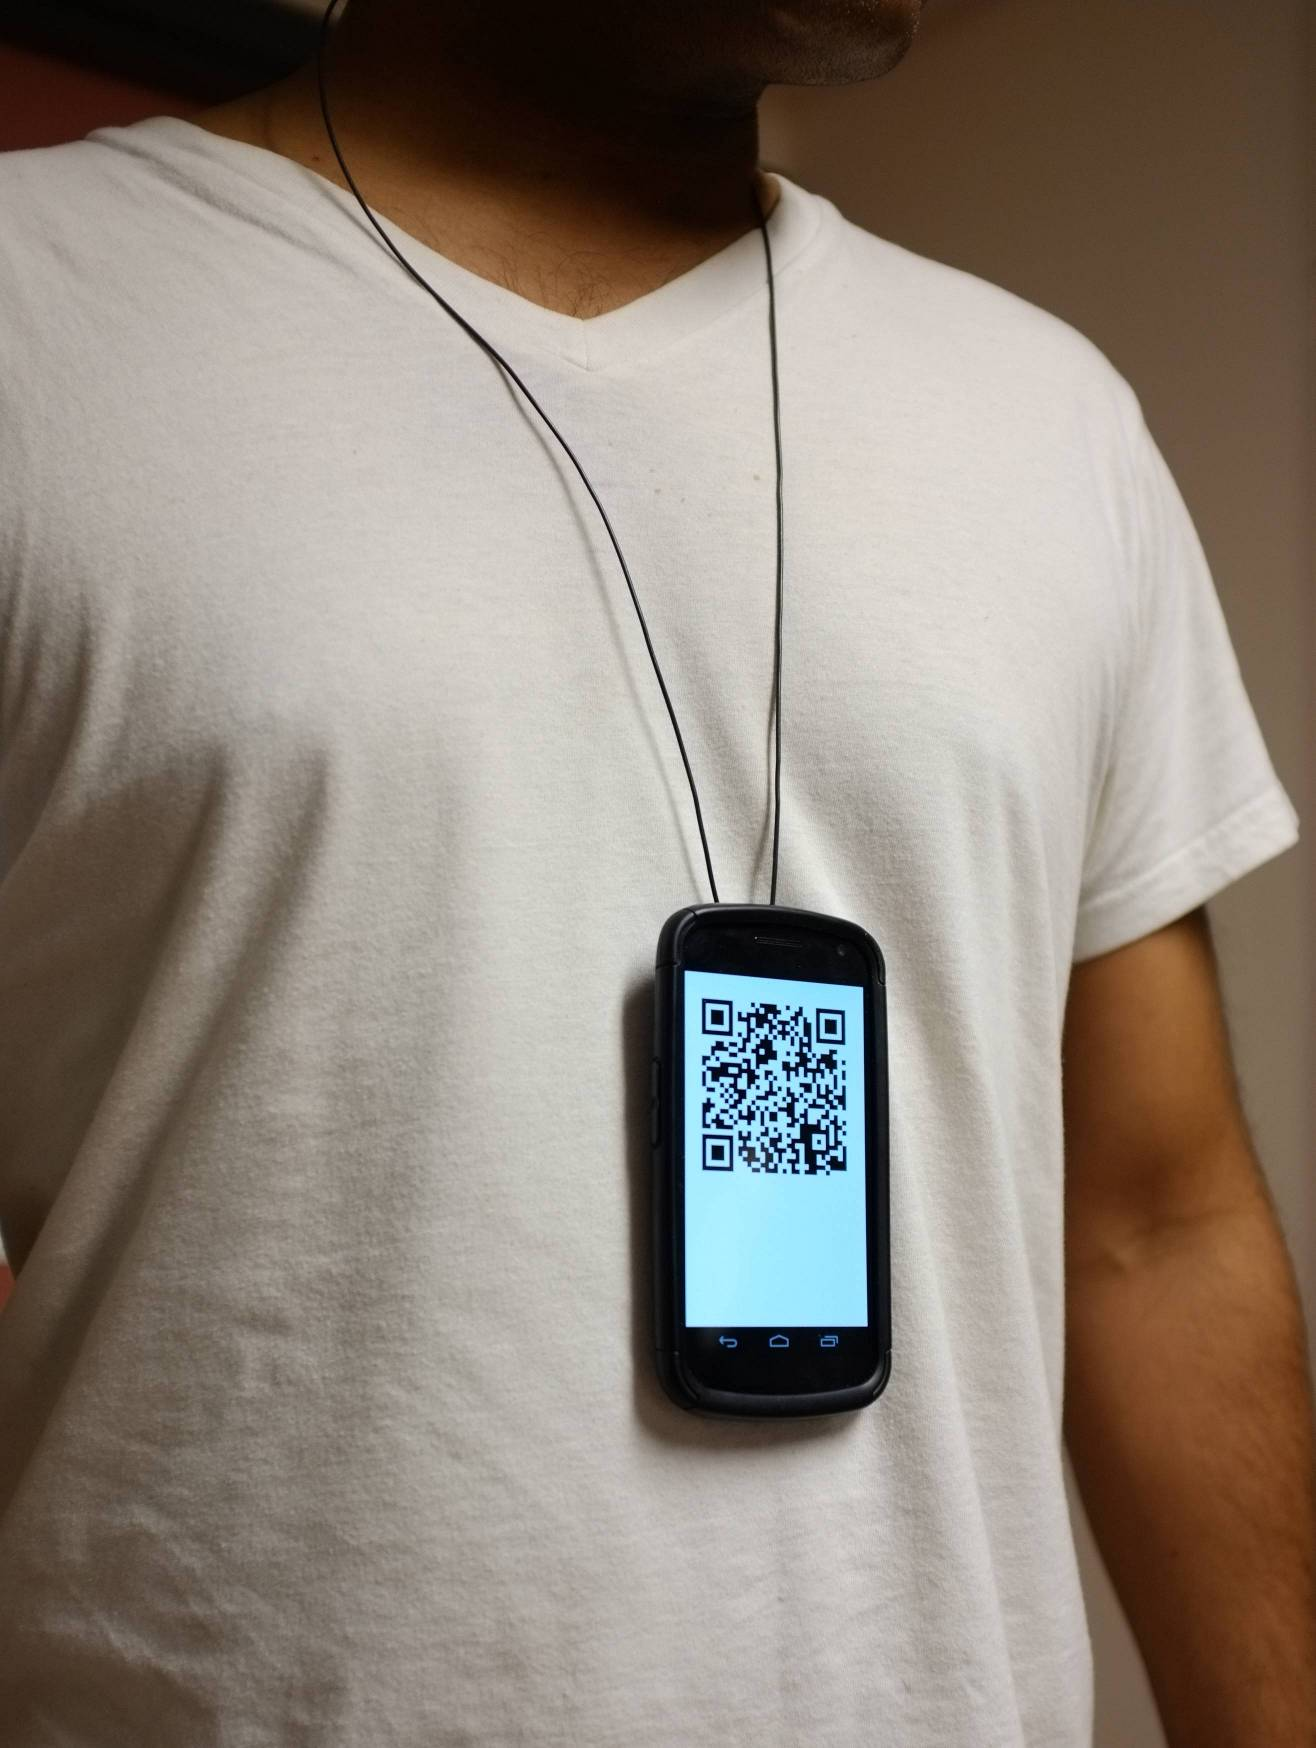
\includegraphics[height=2.0in]{ch6/figs/qr_necklace_und2.jpg} 
    \caption{}
    \label{subfig:qrnecklace}   
\end{subfigure}
  \caption{(a) Video frames from a sousveillance video where a GNU Linux
           wristwatch is seen in-frame.  The barcode display shows the
           latest BITCOIN hash, which --- like the day's news --- is
           difficult to predict, and due to the glare of the watchface, it
           is very difficult to falsify the video by editing it.
           (b) A neck-worn display used to visibly advertise a temporal code
           for the benefit of other parties subjecting us to surveillance
           or sousveillance.
          %, so subsequent timestamping
           %of this video will prove it was taken at the exact moment it
           %was actually taken.
    %Still using a passive display, we can visibly advertise a
    %temporal code for the benefit of other parties subjecting us to
    %surveillance.  This passive display can also incorporate identity
    %information, such as a badge number for emergency personnel,
    %first-responders, and meter-readers. If any of those parties
    %wished to post-date their video, they would need to (a) modify
    %their own recordings, (b) conspire with any other individuals who also
    %obtained video of the same subject matter at the same time, and (c)
    %conspire with the authority (e.g. building owner, police, or government)
    %conducting surveillance of the general area.
}
  \label{fig:wristcomp}   
\end{figure*}
Another possible embodiment is a necklace that displays the current-events
QR hashcode.  See Fig~\ref{subfig:qrnecklace}.

%\begin{figure}
%  \subfigure[]{
%  \includegraphics[height=1in]{ch6/figs/vvs.jpg} 
%  \label{fig:vvs}   
%  }
%  \subfigure[]{
%  \includegraphics[height=1in]{ch6/figs/swipehash.jpg} 
%  \label{fig:swipehash}   
%
%}
%  \caption{(a) Example of incorporating temporal data into a recording
%    using a \emph{vicarious visual soliloquy}~\cite{mann2004clc}.
%    %Since the natural motions of the user's hand is included in the
%    %recording, this is very difficult to falsify.  For an effective
%    %replay attack the time window is from the time of publication of
%    %the temporal code, to the time of submission of the hash of the
%    %recording to a timestamp service.  This is on order of a few
%    %minutes, which is not enough time at present to realistically
%    %render a simulated human hand performing a fairly complex task.  
%   (b) A touchscreen device provides a means to incorporate
%    temporal data into the recorded signal that is nearly foolproof,
%    %since the device guides the user's hand gestures, and reports when
%    %the code is entered correctly.  The range of motions used make
%    %this temporal code injection method difficult to forge, while
%    %providing ease-of-use and secure knowledge that the code has
%    %entered the visual record correctly.
%}
%\end{figure}

\subsection{Visual Vicarious Soliloquy}
Another approach is for the user to occasionally write out or self-gesture
the hash code.  A recording, from a wearable camera, of
one writing out a temporal code in one's own handwriting
is hard to fake.

The challenge here for would-be attackers, is convincingly simulating
an actual, recognizable human hand performing a relatively complex
task of writing out a hash number.  The window of time in which the
attack can take place is bounded in the past by the time the
``headline'' is published, and bounded in the future by the time the
video frames are presented to a digitally signed timestamp server.
This window is on order of a few minutes, which at present is not
enough time for any system known to the authors to perform the
required calculations.

Regarding this limitation, it does require that any claim against the
veracity of the timestamp would also have to address multiple issues
that can leave a forensic trail.  For example, how the simulated hand
was computed, which at present requires a high level of skill and
knowledge, and more computing power than is available to most
individuals.

\subsection{ALIBEye}
\begin{figure}
  \center
  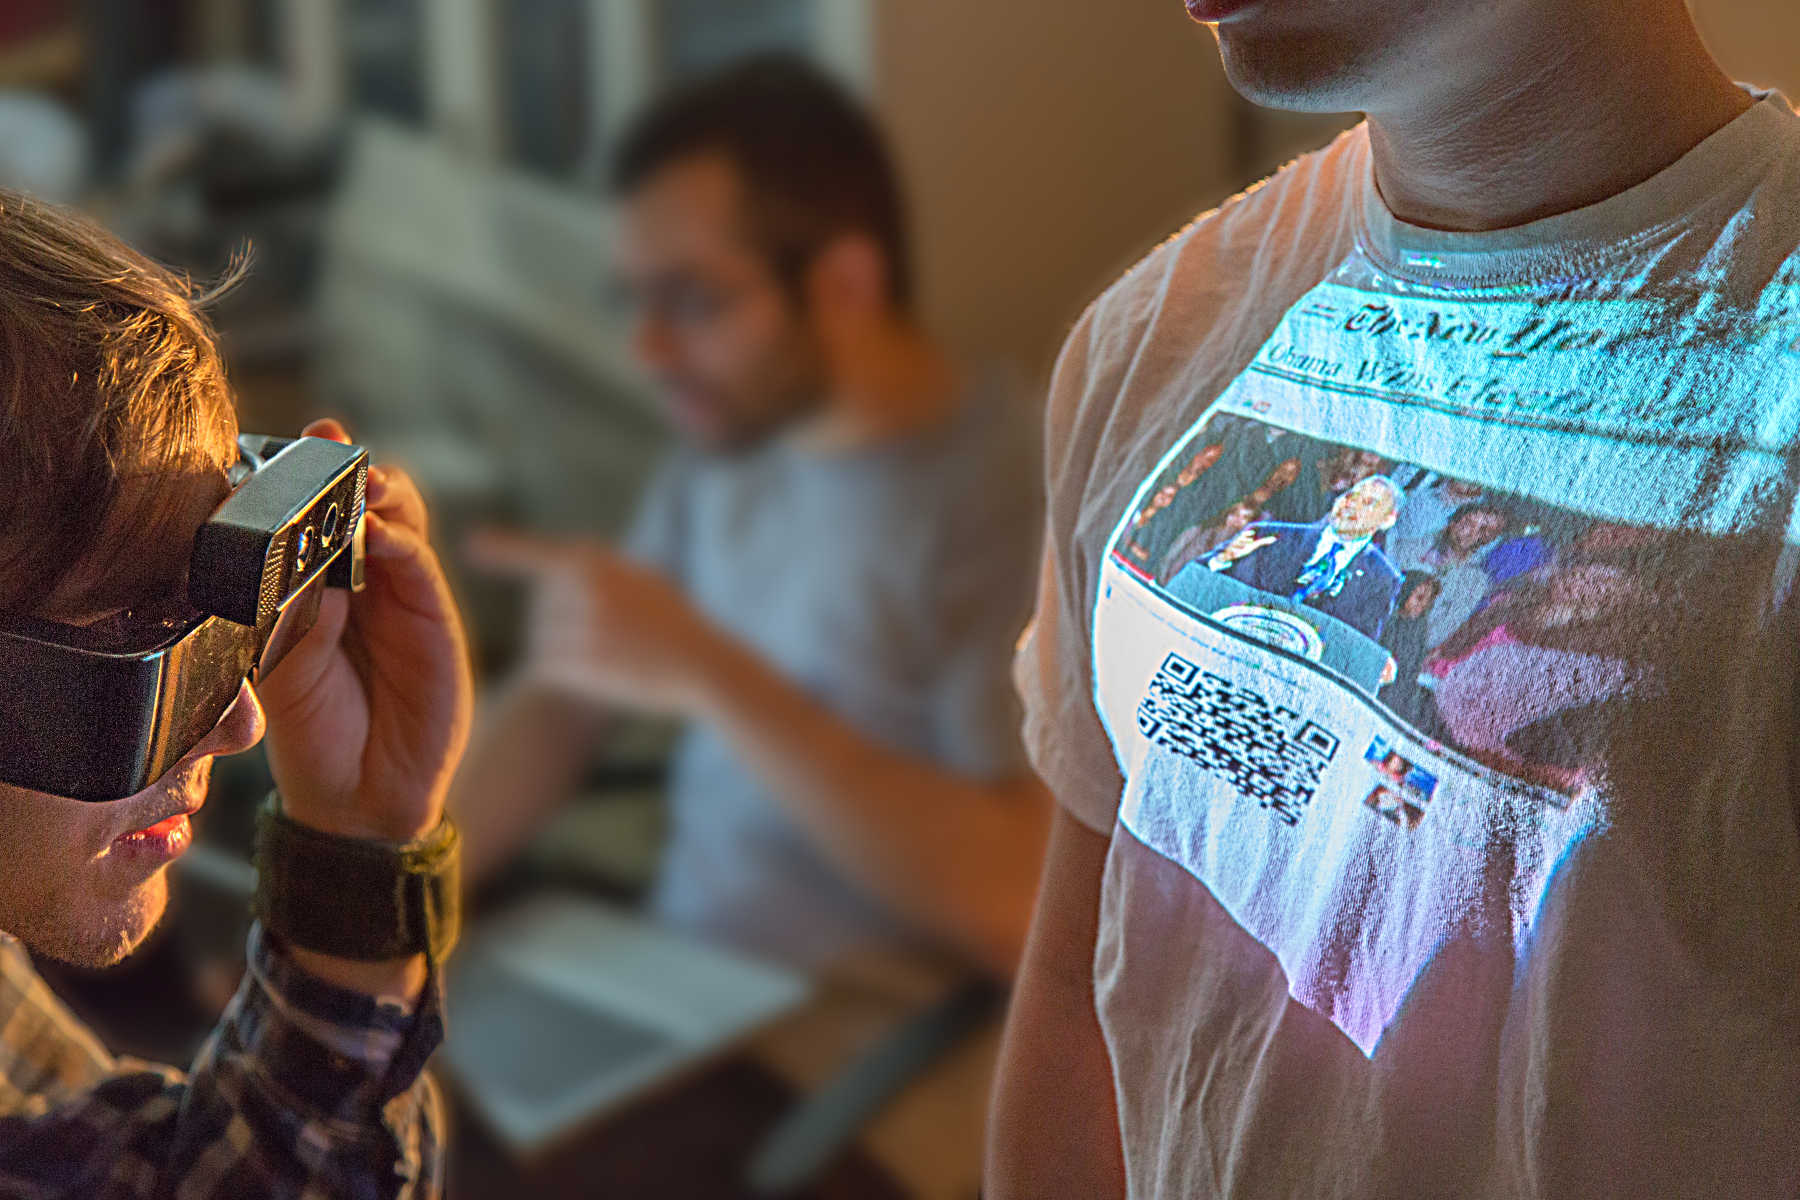
\includegraphics[width=5.2in]{ch6/figs/NYTimes_alibi_veillance_lowres.jpg}
  \caption{A demonstration of the ALIBEye app using a ``News Flash''
           with the Gen-5 Glass.
           A current news headline (Obama's Victory Speech) and a
           2D bar-code are flashed (briefly projected) onto the environment
           (e.g., another person's shirt) to create a NEWStamp$^{TM}$
           that can be seen and recorded
           by the wearer and by others.  The flash duration can be short
           enough to be invisible to the naked eye, but only seen by
           one or more cameras (including the wearer's camera)
           wirelessly synchronized to the ``News Flash''.}
  \label{fig:proj_ray}
\end{figure}

ALIBEye is an app that uses Gen-5 Glass to project a pattern (visible or
infrared) onto the scene and captures recordings of
that pattern, as shown in Fig~\ref{fig:proj_ray}.
The barcode can also include a hash of a recording of the wearer's own
eye, iris pattern, gaze, or eye movements to further bio-metrically
establish their presence in the scene.
The resulting complex interaction is difficult to falsify.
ALIBEye requires little to no attention from the user and
generates continuous automatic updates to the latest temporal code,
which provides safety and security benefits to others, in addition to the wearer.
%Not every frame will provide a machine-readable QR code.
%However, if a significant time has passed since a code was
%successfully recognized, the user can be alerted unobtrusively via
%a Digital Eye Glass system so they can orient themselves in such a manner that a
%successful temporal code recognition can occur.


%extramission glass
%
%VandaLIES
%SigNATURE: NUI-based signature,
%extramissive domewear write long exposure laser pointer QR codes.
%
%counterveillance: 1 strategies: write=camover
%                                data=VanadaLIES.
%Surveillance Camera Players
%Zanta
%
%extramission dome (ece516 telepointer)


\section{Conclusion}
We have described a simple easy-to-build ``FreeGlass'' Generation-5
Digital Eye Glass system along with applications that provide useful interactions and can also
mitigate the one-sided
effects of surveillance.  In one application, the Generation-5 Glass works as
a truly interactive self-gesture-sensing apparatus.  Another application,
``ALIBeye'' (Eyeworn Alibi Veillance), was presented, to make it
difficult for the wearer to falsify the timestamp of a sousveillance
recording.  Sousveillance is not anti-surveillance, and, in fact,
ALIBEye can even facilitate a cooperation between sousveillance and
surveillance so that neither party can falsify
the veracity or time-stamp of their veillance recordings.

